% =====================================================================
%  PACOTE OVERLEAF — Estrutura Produtiva do Espirito Santo (ABNT)
%  Upload no Overleaf: New Project -> Upload Project. Compilador: pdfLaTeX.
%  Arquivo principal: main.tex. Figuras vetoriais em figs/ (PDF).
%
%  Versao: base do autor (alteracoes de 21/07) + revisao linguistica e
%  rediagramacao ABNT (29/07). 44 referencias. Resumo apenas em PT-BR
%  (o abstract em ingles foi retirado a pedido do autor).
%  Versao cega: trocar anonfalse por anontrue.
%
%  DIAGRAMACAO (NBR 14724 + Normas de Apresentacao Tabular do IBGE):
%    - titulo ACIMA do flutuante, com travessao: "Tabela 1 -- ..."
%    - fonte ABAIXO, em corpo menor, alinhada a esquerda
%    - tabela = dados numericos, laterais ABERTAS (booktabs, sem fios verticais)
%    - quadro = conteudo qualitativo, FECHADO por fios (ver Quadro 1)
%
%  Referencias: ABNT NBR 6023:2018 (lista) + NBR 10520:2023 (citacoes
%  autor-data via natbib round/authoryear). Os rotulos opcionais dos
%  bibitem controlam as citacoes — nao remover.
%
%  Tabelas geradas por script — NAO editar a mao, rodar o gerador:
%    tab_multiplicadores.tex  <- pesquisa/27_tab_multiplicadores.py
%    tab_setores.tex          <- pesquisa/12_tab_setores.py
%
%  Pipeline reprodutivel, fixado no commit 116a350:
%  github.com/fcarva/es-insumo-produto
%  NOTA: paper/es_estrutura_produtiva.tex ficou numa revisao anterior
%  (com o apendice de escores-z do modelo nulo, a tabela de benchmark
%  ampliada e as figuras de upstreamness/fractal, que esta versao nao
%  usa); este arquivo e a versao de trabalho desta rodada.
% =====================================================================
\documentclass[11pt,a4paper]{article}
\PassOptionsToPackage{hyphens}{url} % quebra URLs longas antes do hyperref
\usepackage[utf8]{inputenc}
\usepackage[T1]{fontenc}
\usepackage{lmodern}
\usepackage[brazilian]{babel}
\usepackage{microtype}
\usepackage{amsmath,amssymb}
\usepackage{array}
\usepackage{booktabs}
\usepackage{graphicx}
\usepackage{geometry}
\usepackage{xcolor}
\usepackage[flushleft]{threeparttable}
\usepackage{newfloat}
\usepackage[font=small,labelfont=bf,labelsep=endash,
            justification=raggedright,singlelinecheck=false]{caption}
\usepackage[round,authoryear]{natbib}
\usepackage[hidelinks]{hyperref}
\geometry{margin=2.5cm}

% Versão cega para avaliação por pares: trocar por \anontrue antes de compilar
\newif\ifanon
\anonfalse
\graphicspath{{figs/}}

% --- Flutuante "Quadro": conteúdo qualitativo, fechado por fios (ABNT) ---
\DeclareFloatingEnvironment[name=Quadro,fileext=loq,placement=tbp]{quadro}

% --- Fonte sob ilustrações (as tabelas usam tablenotes do threeparttable) ---
\newcommand{\fonte}[1]{%
  \par\vspace{3pt}%
  \begin{minipage}{\linewidth}\footnotesize\raggedright #1\end{minipage}\par}

% TODO EDITORIAL (A9): o subtítulo diz "demanda" (vago -> "decomposição da demanda
% final") e "composição territorial da indústria", mais estreito que a seção 6, que
% cobre agropecuária, rochas, têxtil e serviços -> bastaria "composição territorial".
\title{\textbf{Estrutura Produtiva do Espírito Santo:\\ uma análise de insumo-produto}\\[2pt]
\large Multiplicadores, setores-chave, demanda, composição territorial da indústria e a face
plataforma de uma economia de base (2008--2021)}
\author{\ifanon Autor omitido para avaliação cega\else Felipe Carvalho\\
\small PPGEco --- UFES \quad$\cdot$\quad Análise de Insumo-Produto --- Prof. Dr. Celso Bissoli Sessa\\
% TODO: substituir pelo ORCID real e, se houver, pelo e-mail institucional antes do envio
\small ORCID: 0009-0008-8578-9018 \quad$\cdot$\quad
\texttt{felipe.c.santos@edu.ufes.br}\fi}
\date{julho de 2026}

\begin{document}
\maketitle
\thispagestyle{empty}

\begin{abstract}
\noindent
Este artigo caracteriza a estrutura produtiva do Espírito Santo (ES) pela ótica da análise de
insumo-produto, na tradição brasileira de estudo de economias estaduais, combinando a
matriz inter-regional ES\,$\times$\,restante do Brasil de 2008 (26 setores, com vetor de emprego),
a série nacional de 68 setores (2010--2021) e o sistema inter-regional das dez
microrregiões de planejamento (2015). O retrato é o de uma \emph{economia de base dual}:
os setores líderes, como mineração, petróleo, siderurgia e celulose, concentram
encadeamento (as maiores ligações puras), mas geram pouco emprego e pouca renda direta;
a extração opera como \emph{enclave}; a transformação, como setor-chave. A decomposição pela
demanda final quantifica o descolamento: a demanda externa ao estado induz \textbf{61,7\%}
da produção, mas apenas 47,5\% do emprego. Um \emph{benchmark} com as 27 unidades da federação
mostra que a dualidade é genérica em tipo, mas extrema em grau. O ES é o segundo estado
mais intensivo em setores de base. No território, um núcleo metropolitano diversificado que
retém 90,9\% de seu multiplicador contrasta com periferias especializadas que vazam; pelo lado
da abertura, o encadeamento escoa ao núcleo São Paulo--Rio com \emph{feedback} quase nulo.

\vspace{0.6em}
\noindent\textbf{Palavras-chave:} insumo-produto; estrutura produtiva; multiplicadores;
setores-chave; economia regional; Espírito Santo.

\noindent\textbf{Códigos JEL:} R15; D57; C67.

\vspace{1.1em}
\end{abstract}
% =====================================================================
\section{Introdução}
\label{sec:intro}
% TODO EDITORIAL (A8): os dois números abaixo (2\% do produto nacional; um quarto do
% produto estadual) e o advérbio "hoje" precisam de fonte e de ano de referência —
% Contas Regionais do IBGE. Num artigo cuja matriz é de 2008, "hoje" fica indefinido.
O Espírito Santo respondia, em 2008, por cerca de 2\% do produto nacional, mas sua
estrutura produtiva é atípica: pequena, aberta e organizada em torno de setores de base
intensivos em \emph{commodities}: minério de ferro e pelotização, siderurgia, petróleo e gás,
celulose e rochas ornamentais. Em quatro décadas, a economia capixaba mudou de motor duas
vezes: da monocultura cafeeira para a indústria de base nos anos 1980 (os grandes projetos
siderúrgicos, de celulose e de pelotização) e, a partir do fim dos anos 1990, para o petróleo,
que hoje representa cerca de um quarto do produto estadual.

A literatura brasileira de insumo-produto consolidou um formato para \emph{caracterizar}
uma economia estadual: a partir de uma matriz inter-regional (estado \emph{versus}
restante do país), computam-se multiplicadores, ligações intersetoriais e
setores-chave, identificando o perfil de especialização e os centros de dinamismo.
A \S\ref{sec:quadro} organiza uma revisão de literatura sob a ótica da teoria do
desenvolvimento regional para situar o Espírito Santo no debate nacional.

Para o Espírito Santo, há contribuições pontuais: \citet{sessa2017ubu} avaliam o impacto
socioeconômico de um projeto siderúrgico (Ubu, Anchieta) pela matriz capixaba, e
\citet{ribeiro2024dinamica} regionalizam a matriz de 2015 nas dez microrregiões de
planejamento, computando multiplicadores de produção, emprego e renda.

Falta, contudo, uma caracterização estrutural que reúna a bateria completa de indicadores e a
situe num \emph{benchmark} interestadual, capaz de distinguir o que na economia capixaba é
regularidade do que lhe é peculiar.
% TODO EDITORIAL (A2): o roteiro abaixo anuncia quatro perguntas — a quarta foi
% acrescentada porque a seção 7 (abertura e face plataforma) está no título, no resumo
% e na conclusão, mas não aparecia no roteiro. Confirmar a redação.
Este artigo busca responder a quatro perguntas: (i) \emph{que tipo de economia} é o ES:
quais são seus multiplicadores, setores-chave e polos de crescimento, e \emph{quem puxa}
sua produção e seu emprego (\S\ref{sec:retrato});
(ii) \emph{como} a posição estrutural de seus setores de base evoluiu
(\S\ref{sec:panorama}); (iii) \emph{qual a composição industrial} de cada um de seus
territórios (\S\ref{sec:territorio}); e (iv) \emph{como} o encadeamento que ele gera se
reparte entre o que fica no estado e o que escoa ao núcleo industrial brasileiro
(\S\ref{sec:plataforma}). A contribuição não é testar uma hipótese, mas oferecer um retrato
insumo-produto da economia do Espírito Santo.

% =====================================================================
\section{Revisão de literatura: a teoria regional na ótica de insumo-produto}
\label{sec:quadro}
Três lentes da teoria do desenvolvimento regional organizam a leitura que este artigo faz da
economia do Espírito Santo, e cada uma tem tradução direta na análise de insumo-produto
(Quadro~\ref{qua:lentes}). A primeira é a \emph{base de exportação}: o crescimento de uma
economia regional é comandado pela demanda externa à região \citep{north1955}, ao que
\citet{tiebout1956} contrapôs o peso das atividades residentes, voltadas ao mercado interno,
na ocupação e no multiplicador local. \citet{richardson1985} formalizou a ponte com o método:
o multiplicador de base econômica é o caso agregado do multiplicador insumo-produto, que o
desagrega setor a setor. A lente se operacionaliza aqui na decomposição da produção e do
emprego segundo os componentes da demanda final --- que mede diretamente \emph{quem puxa} a
economia (\S\ref{sec:retrato}) --- e no fechamento de tipo II, que endogeneiza o circuito
induzido pelos residentes.

A segunda lente é a dos \emph{polos de crescimento}: o crescimento não aparece em toda
parte ao mesmo tempo, mas em \emph{indústrias motrizes} que o irradiam pelos encadeamentos
\citep{perroux1955}; \citet{hirschman1958} deu ao mecanismo sua métrica, as ligações para trás
e para frente que induzem investimento a montante e a jusante, e \citet{rasmussen1956}, sua
normalização. A operacionalização é dupla: os índices de Rasmussen--Hirschman, neutros em
relação ao porte, identificam os \emph{setores-chave}; as ligações puras
\citep{cella1984,guilhoto2005linkages} reintroduzem o porte e identificam os polos de
crescimento de Perroux (\S\ref{sec:retrato}).

A terceira lente é a da \emph{interdependência centro-periferia}. Na linguagem
inter-regional inaugurada por \citet{isard1951}, o encadeamento de uma região reparte-se entre
o que ela retém e o que transborda (\emph{spillover}); \citet{miller1966} mostrou que o retorno
(\emph{feedback}) é tipicamente pequeno, e \citet{miyazawa1966} decompôs o mecanismo em
multiplicadores internos e externos. Na tradição brasileira, essa mecânica tem leitura
estrutural: o ES como periferia do núcleo industrial brasileiro \citep{cano1985}, numa
hierarquia de núcleos e periferias que se repete em escalas aninhadas \citep{friedmann1966}.
Operacionalizam-na a partição de Isard (vazamento, \emph{spillover}, \emph{feedback}) e a
extração hipotética \citep{dietzenbacher1993} (\S\ref{sec:territorio}--\S\ref{sec:plataforma}).
As três lentes são, no fim, três leituras do mesmo sistema $x=(I-A)^{-1}y$: a primeira pergunta
quem move $y$; a segunda, como a inversa propaga o impulso; a terceira, \emph{onde} o
encadeamento se realiza.

\begin{quadro}[tbp]
\caption{As três lentes da teoria do desenvolvimento regional e sua tradução insumo-produto
neste artigo}
\label{qua:lentes}
\centering\small
\renewcommand{\arraystretch}{1.2}
\begin{tabular}{|>{\raggedright\arraybackslash}p{3.2cm}|>{\raggedright\arraybackslash}p{5.5cm}|>{\raggedright\arraybackslash}p{5.5cm}|}
\hline
\textbf{Lente teórica} & \textbf{Instrumento insumo-produto} & \textbf{Onde o artigo mede}\\
\hline
\textbf{Base de exportação}\newline{\footnotesize North (1955); Tiebout (1956); Richardson (1985)}&
decomposição da produção e do emprego pela demanda final; multiplicadores de tipo II &
\S\ref{sec:retrato}: a demanda externa puxa 61,7\% da produção, mas 47,5\% do emprego;
mult.\ de emprego 27,9$\,\to\,$40,4 no tipo II\\
\hline
\textbf{Polos de crescimento}\newline{\footnotesize Perroux (1955); Hirschman (1958); Rasmussen (1956)} &
índices de Rasmussen--Hirschman; ligações puras (GHS) &
\S\ref{sec:retrato}: setores-chave concentrados na transformação; polos mineração (4,4) e
metalurgia (3,4)\\
\hline
\textbf{Centro-periferia}\newline{\footnotesize Isard (1951); Miller (1966); Miyazawa (1966); Friedmann (1966); Cano (1985)} &
partição inter-regional (\emph{spillover} e \emph{feedback}); extração hipotética &
\S\ref{sec:territorio}--\S\ref{sec:plataforma}: retenção de 90,9\% (núcleo) a 66,2\%
(periferia); \emph{feedback} de 0,32\%; extração da metrópole: $-13{,}0$\%\\
\hline
\end{tabular}
\fonte{Fonte: elaboração própria.}
\end{quadro}

É nesse quadro que se consolidou, no Brasil, o gênero ``estrutura produtiva'': Minas Gerais
inaugurou o desenho bi-regional \citep{domingues2002matriz}, seguido de Mato Grosso
\citep{figueiredo2004agriculture}, Rio Grande do Sul \citep{porsse2008matriz}, Pará
\citep{sessofilho2010para} --- e, em Santa Catarina, a leitura da indústria estadual sobre a
MIP de 2018 \citep{bittencourt2023sc}; o recorte multiestadual tem precedente no sistema
inter-regional do Nordeste \citep{guilhoto2010nordeste} e o recorte intra-estadual, no sistema
dos municípios paulistas \citep{ichihara2008geo}. Este artigo traz esse formato ao Espírito
Santo e lhe acrescenta um \emph{benchmark} interestadual, que busca separar o que é
regularidade do que é especificidade na estrutura produtiva capixaba.

% =====================================================================
\section{Metodologia}
\label{sec:metodo}
\subsection{Dados: as matrizes utilizadas}
\label{sec:dados}
A análise combina três fontes, todas processadas por rotinas
reprodutíveis\footnote{Todo o pipeline --- scripts, séries intermediárias, arquivos de saída e
figuras vetoriais --- está versionado em \url{https://github.com/fcarva/es-insumo-produto}. Os
links das fontes de tabelas e figuras deste artigo apontam para o \emph{commit}
\texttt{116a350}, que fixa o estado exato do código que gerou cada resultado aqui reportado
\citep{carvalho2026repo}.}: (a) a matriz \textbf{inter-regional ES\,$\times$\,restante do
Brasil} de 2008, 26 setores por região, em R\$ milhões correntes, balanceada e
acompanhada dos vetores de remunerações e de pessoal ocupado, que sustenta o retrato
estrutural; (b) a \textbf{série nacional de 68 setores} (2010--2021), que permite a leitura
temporal; e (c) o \textbf{sistema inter-regional das dez microrregiões de planejamento do ES}
(2015, 35 setores), que sustenta a caracterização territorial. A construção das matrizes
regionais segue a tradição brasileira de regionalização não censitária da matriz nacional
\citep{guilhoto2005estimacao,round1983nonsurvey} pelo método IIOAS \citep{haddad2017iioas}. As
heterogeneidades de safra (2008/2015) e agregação (26/35/68 setores) e o caráter
\emph{estimado} dos fluxos inter-regionais são discutidos em \S\ref{sec:limites}.

Duas fronteiras ficam deliberadamente fora do escopo empírico central e entram como referência
metodológica e agenda. A primeira é a \textbf{atualização da matriz interestadual brasileira}
de 2019 \citep{haddad2025matriz}, usada apenas como checagem contextual: nela, o ES combina
\emph{déficit} no comércio inter-regional (R\$\,72,7 bi exportados contra R\$\,88,4 bi
importados) com \emph{superávit} no internacional --- padrão compatível com a leitura de
economia aberta deste artigo, mas medido em outra safra e agregação. A segunda é a
regionalização por métodos não censitários alternativos --- quocientes locacionais corrigidos
(FLQ/AFLQ; \citealp{flegg1995lq,flegg2000flq}), sensíveis à calibragem
\citep{flegg2016evaluating}; o método CHARM, que corrige o \emph{cross-hauling}
\citep{tobben2015charm}; as abordagens gravitacionais \citep{riddington2006comparison}; e o
ajuste biproporcional GRAS \citep{junius2003gras} ---, que entra aqui como critério de leitura
da incerteza dos fluxos estimados (\S\ref{sec:limites}); os resultados reportados são os que
remontam diretamente às três matrizes disponíveis.

\subsection{Instrumentos: o modelo e os indicadores}
\label{sec:instrumentos}
O sistema parte da identidade de Leontief $x=(I-A)^{-1}y=By$, com $A=Z\hat{x}^{-1}$.
Sobre $B$ (e, pelo lado da oferta, sobre a inversa de Ghosh $G$) computa-se a bateria
de indicadores que caracteriza uma economia regional \citep{millerblair2009}. Os parágrafos
seguintes resumem cada instrumento; as derivações completas, equação a equação, estão no
Apêndice~\ref{ap:metodologia}.

\paragraph{Multiplicadores.}
O multiplicador de produção do setor $j$ é $O_j=\sum_i b_{ij}$ (Apêndice~\ref{ap:leontief}).
Os de emprego e renda são $E_j=\sum_i w_i b_{ij}$ e $R_j=\sum_i v_i b_{ij}$, com coeficientes
diretos $w_i=\text{ocup}_i/x_i$ e $v_i=\text{rem}_i/x_i$. Os multiplicadores de \emph{tipo II}
fecham o modelo para as famílias \emph{do ES} (renda das remunerações dos setores capixabas;
consumo das famílias capixabas), endogeneizando o efeito-renda induzido. Num sistema
bi-regional, essa escolha fornece um \emph{limite inferior} do induzido capixaba, pois parte do
consumo das famílias se realiza em produtos do restante do Brasil e não retorna como demanda
ao ES.

\paragraph{Decomposição pela demanda final.}
Sendo $x=By$ linear em $y$, a produção (e, via coeficientes diretos, o emprego)
atribuível a cada componente da demanda final é $x^{(k)}=By^{(k)}$, com
$y=\sum_k y^{(k)}$ particionada em exportações internacionais, demanda final do
restante do Brasil, consumo das famílias, governo/ISFLSF, formação bruta de capital e variação
de estoques (Apêndice~\ref{ap:fd}). A soma dos componentes reproduz exatamente $x$; a
decomposição identifica \emph{quem puxa} cada setor.

\paragraph{Ligações e setores-chave.}
Os índices de \citet{rasmussen1956} e \citet{hirschman1958} medem o poder de dispersão (para
trás, pela inversa de Leontief) e a sensibilidade de dispersão (para frente, pela inversa de
Ghosh), normalizados pela média; \emph{setores-chave} têm ambos os índices superiores à
unidade (Apêndice~\ref{ap:rh}). O coeficiente de variação desses índices mede o grau de
integração da economia.

\paragraph{Ligações puras.}
Como a normalização de Rasmussen--Hirschman é insensível ao tamanho do setor, computam-se
também as \emph{ligações puras} \citep{guilhoto2005linkages,millerblair2009}, herdeiras do
método de extração de \citet{cella1984}, que ponderam o encadeamento pela produção do setor.
Particionando a economia em $\{j\}$ e o resto $\{r\}$, a ligação pura para trás é
$\mathrm{PBL}_j=\Delta^{r}A^{rj}\Delta^{j}y_j$ e a ligação pura para frente,
$\mathrm{PFL}_j=\Delta^{j}A^{jr}\Delta^{r}y_r$, com $\Delta^{r}=(I-A^{rr})^{-1}$ e
$\Delta^{j}=(1-a_{jj})^{-1}$; a ligação pura total $\mathrm{PTL}_j$ identifica os verdadeiros
polos de crescimento (Apêndice~\ref{ap:puras}).

\paragraph{Composição territorial.}
A especialização de cada microrregião é medida pelo \emph{quociente locacional}
$\mathrm{LQ}_{gs}=(x_{gs}/\sum_s x_{gs})/(\sum_g x_{gs}/\sum_{gs}x_{gs})$; valores
superiores à unidade indicam que o setor $s$ se concentra no território $g$ mais do que na
média estadual (Apêndice~\ref{ap:lq}).

\paragraph{Abertura: \emph{spillover} e \emph{feedback}.}
Para medir a abertura, particiona-se o sistema em região-foco $L$ e resto $M$, aplicando-se
a decomposição de Isard \citep{isard1951,millerblair2009}. Injetando a demanda final de $L$
por seus próprios produtos, a produção induzida em $M$,
$x^{M}=(I-A^{MM})^{-1}A^{ML}x^{L}$, é o \emph{spillover}; o retorno a $L$ pelo termo de
\emph{feedback} da inversa particionada $(I-A^{LL}-A^{LM}(I-A^{MM})^{-1}A^{ML})^{-1}$ é o
\emph{feedback} (Apêndice~\ref{ap:isard}). A razão \emph{feedback}/injeção, computada em cada
escala (UFs e microrregiões), mede a reciprocidade do encadeamento; a decomposição
multiplicativa de \citet{miyazawa1966} separa, no mesmo particionamento, multiplicadores
internos e externos (Apêndice~\ref{ap:miyazawa}). Complementarmente, a \emph{extração
hipotética} \citep{dietzenbacher1993} remove uma unidade do sistema e mede a produção que
deixaria de existir sem ela (Apêndice~\ref{ap:hem}).

% =====================================================================
\section{O retrato estrutural (2008)}
\label{sec:retrato}
\paragraph{Multiplicadores.}
A Tabela~\ref{tab:mult} reporta a bateria completa de multiplicadores --- produção,
emprego e renda, tipos I e II --- dos 26 setores. O multiplicador de produção médio é
1,76 (tipo I) e 2,45 (tipo II). Os mais altos estão na indústria de transformação ---
alimentos (2,31), refino (2,11), material de transporte (2,10) e químicos (2,10). O
contraste com os multiplicadores de \emph{emprego} é o achado central do retrato: a
geração de empregos (média de 27,9 por R\$ 1 milhão de demanda final, no tipo I) concentra-se
em setores intensivos em trabalho --- têxtil (67,9), pecuária (57,0), alojamento (50,2),
serviços (49,2) e agricultura (46,7) ---, \emph{nenhum} deles um setor de base.

A geração de renda das famílias, por sua vez, é maior em educação, administração
pública, saúde e serviços. Os setores que lideram a economia capixaba não são os que mais
empregam nem os que mais distribuem renda diretamente.

\begin{table}[tbp]
\caption{Multiplicadores de produção, emprego e renda dos 26 setores do ES, tipos I e II
(2008)}
\label{tab:mult}
\centering\footnotesize
\begin{threeparttable}
\begin{tabular}{lrrrrrr}
\toprule
& \multicolumn{2}{c}{Produção} & \multicolumn{2}{c}{Emprego} & \multicolumn{2}{c}{Renda}\\
\cmidrule(lr){2-3}\cmidrule(lr){4-5}\cmidrule(lr){6-7}
Setor & Tipo I & Tipo II & Tipo I & Tipo II & Tipo I & Tipo II\\
\midrule
Alimentos/bebidas/fumo & 2,31 & 2,79 & 42,5 & 51,2 & 0,201 & 0,252\\
Refino/coque/álcool & 2,11 & 2,49 & 21,7 & 28,5 & 0,157 & 0,197\\
Material de transporte & 2,10 & 2,73 & 16,0 & 27,3 & 0,262 & 0,328\\
Químicos/farmacêuticos & 2,10 & 2,52 & 13,3 & 20,8 & 0,174 & 0,218\\
Borracha/plástico & 2,05 & 2,64 & 19,9 & 30,5 & 0,245 & 0,307\\
Máquinas/equip. & 2,00 & 2,71 & 17,2 & 30,0 & 0,294 & 0,368\\
Mat. elétrico/eletrônicos & 1,99 & 2,61 & 15,5 & 26,7 & 0,260 & 0,326\\
Madeira/papel & 1,96 & 2,39 & 21,9 & 29,7 & 0,179 & 0,224\\
Metalurgia & 1,96 & 2,34 & 11,3 & 18,2 & 0,158 & 0,199\\
Min. não-metálicos & 1,90 & 2,54 & 23,1 & 34,8 & 0,268 & 0,336\\
Têxtil/vestuário & 1,87 & 2,45 & 67,9 & 78,3 & 0,240 & 0,301\\
Indústrias diversas & 1,84 & 2,27 & 40,3 & 48,1 & 0,180 & 0,226\\
Eletricidade/gás/água & 1,83 & 2,23 & 11,6 & 18,7 & 0,165 & 0,206\\
Transporte/armazenagem & 1,77 & 2,55 & 22,4 & 36,5 & 0,325 & 0,407\\
Alojamento/alimentação & 1,76 & 2,31 & 50,2 & 60,2 & 0,229 & 0,287\\
Construção & 1,70 & 2,25 & 30,1 & 40,1 & 0,231 & 0,289\\
Pecuária e pesca & 1,64 & 2,60 & 57,0 & 74,5 & 0,403 & 0,505\\
Mineração & 1,64 & 1,98 & 10,1 & 16,2 & 0,142 & 0,178\\
Saúde & 1,54 & 2,90 & 28,7 & 53,4 & 0,571 & 0,716\\
Serviços privados & 1,50 & 2,53 & 49,2 & 67,8 & 0,430 & 0,540\\
Financeiro/seguros & 1,47 & 2,32 & 12,7 & 28,1 & 0,355 & 0,446\\
Agricultura/silvicultura & 1,45 & 1,95 & 46,7 & 55,6 & 0,206 & 0,258\\
Adm. pública & 1,43 & 2,97 & 19,5 & 47,4 & 0,644 & 0,808\\
Comércio & 1,42 & 2,29 & 36,9 & 52,6 & 0,362 & 0,454\\
Educação & 1,31 & 3,17 & 33,6 & 67,3 & 0,778 & 0,976\\
Imobiliário/aluguel & 1,15 & 1,27 & 6,3 & 8,5 & 0,051 & 0,064\\
\midrule
\textbf{Média (simples)} & 1,76 & 2,45 & 27,9 & 40,4 & 0,289 & 0,362\\
\bottomrule
\end{tabular}

\begin{tablenotes}[flushleft]\footnotesize
\item Nota: setores ordenados pelo multiplicador de produção de tipo I. Emprego em empregos
por R\$\,1 milhão de demanda final; renda em R\$ por R\$\,1 de demanda final.
\item Fonte: elaboração própria a partir de
\href{https://github.com/fcarva/es-insumo-produto/blob/116a350/pesquisa/27_tab_multiplicadores.py}{\texttt{27\_tab\_multiplicadores.py}}
sobre
\href{https://github.com/fcarva/es-insumo-produto/blob/116a350/pesquisa/outputs/es_caracterizacao_2008.csv}{\texttt{outputs/es\_caracterizacao\_2008.csv}}
\citep{carvalho2026repo}.
\end{tablenotes}
\end{threeparttable}
\end{table}

\paragraph{Quem puxa a economia: a decomposição pela demanda final.}
A mesma assimetria aparece ao perguntar \emph{de onde vem} a demanda que sustenta a
produção capixaba (Tabela~\ref{tab:decomp}). A demanda \textbf{externa ao estado}
--- exportações internacionais (29,1\%) e demanda final do restante do Brasil (32,7\%)
--- induz, direta e indiretamente, \textbf{61,7\%} da produção do ES, mas apenas
\textbf{47,5\%} do emprego; o consumo das famílias capixabas, com 18,8\% da produção,
carrega 25,7\% do emprego, e o governo, com 13,1\% da produção, responde por 16,1\% do
emprego. O contraste setorial é nítido: refino, metalurgia, mineração e madeira/papel são
puxados quase integralmente de fora (mais de 96\% da produção induzida por demanda
externa\footnote{No refino, a parcela externa excede 100\% (138,6\%) porque a variação de
estoques é negativa; a soma dos componentes reproduz exatamente a produção total (checagem em
\href{https://github.com/fcarva/es-insumo-produto/blob/116a350/pesquisa/25_decomposicao_fd.py}{\texttt{25\_decomposicao\_fd.py}}).}),
enquanto administração pública, educação e saúde dependem em 90\% ou mais da demanda
doméstica. A economia de base é, portanto, uma economia \emph{puxada de fora}: o motor da
produção está no resto do país e no exterior, mas o emprego que esse motor gera fica, em boa
parte, aquém do seu peso na produção --- é o mercado interno que emprega. É a fotografia
insumo-produto da \emph{base de exportação} (\S\ref{sec:quadro}): a demanda externa comanda o
crescimento da produção, e a ressalva de \citet{tiebout1956} reaparece pelo lado do emprego ---
são as atividades \emph{residentes}, voltadas ao mercado interno, que carregam a ocupação. O
canal de Tiebout é visível no próprio fechamento do modelo: os multiplicadores de tipo~II ---
que endogeneizam o consumo das famílias capixabas --- elevam o multiplicador médio de emprego
de 27,9 para 40,4 empregos por R\$\,1 milhão; é nesse circuito induzido, doméstico, que as
atividades residentes se sustentam.

\begin{table}[tbp]
\caption{Produção e emprego do ES atribuídos a cada componente da demanda final (2008)}
\label{tab:decomp}
\centering\small
\begin{threeparttable}
\begin{tabular}{lrrrr}
\toprule
Componente da demanda final & Produção (R\$ bi) & \% & Emprego (mil) & \% \\
\midrule
Demanda final do restante do Brasil & 34,2 & 32,7 & 477,8 & 29,6 \\
Exportações (resto do mundo) & 30,4 & 29,1 & 287,8 & 17,9 \\
Consumo das famílias ES & 19,7 & 18,8 & 414,5 & 25,7 \\
Governo + ISFLSF ES & 13,7 & 13,1 & 259,4 & 16,1 \\
Formação bruta de capital ES & 7,6 & 7,3 & 163,7 & 10,2 \\
Variação de estoques ES & $-1,0$ & $-1,0$ & 8,6 & 0,5 \\
\midrule
\textbf{Total} & \textbf{104,6} & \textbf{100,0} & \textbf{1.611,7} & \textbf{100,0} \\
\bottomrule
\end{tabular}
\begin{tablenotes}[flushleft]\footnotesize
\item Nota: produção e emprego atribuídos via $x^{(k)}=By^{(k)}$. A demanda externa ao estado
(duas primeiras linhas) puxa 61,7\% da produção, mas 47,5\% do emprego.
\item Nota: as parcelas externas somam 61,75\% antes do arredondamento --- somar as duas
primeiras linhas da coluna de percentuais, já arredondadas, resulta em 61,8. O mesmo vale para
o total de emprego (1.611,7 mil no agregado; 1.611,8 se somadas as parcelas arredondadas).
\item Fonte: elaboração própria a partir de
\href{https://github.com/fcarva/es-insumo-produto/blob/116a350/pesquisa/25_decomposicao_fd.py}{\texttt{25\_decomposicao\_fd.py}}
sobre
\href{https://github.com/fcarva/es-insumo-produto/blob/116a350/pesquisa/outputs/decomposicao_fd.csv}{\texttt{outputs/decomposicao\_fd.csv}}
\citep{carvalho2026repo}.
\end{tablenotes}
\end{threeparttable}
\end{table}

\paragraph{Setores-chave e polos de crescimento.}
Pela classificação de Rasmussen--Hirschman, os setores-chave (ambos os índices acima de
1) concentram-se na cadeia industrial de transformação: refino, químicos, borracha/plástico,
cimento e minerais não metálicos, metalurgia, material elétrico, material de transporte
e eletricidade/gás/água (Figura~\ref{fig:chave}). Chama atenção que a mineração tenha
\emph{ligação para frente} elevada ($\approx1{,}2$), mas \emph{ligação para trás}
baixa ($\approx0{,}9$): é fornecedora a montante, não setor-chave pleno --- a
assinatura de um \emph{enclave} que compra pouco internamente. Já as ligações puras,
ponderadas por tamanho, identificam os verdadeiros polos: \textbf{mineração}
($\mathrm{PTL}$ padronizado 4,4) e \textbf{metalurgia} (3,4) à frente, seguidas de
transporte, comércio e serviços.\footnote{A ligação pura total correlaciona-se fortemente
com o valor bruto da produção (Pearson 0,96): é, sobretudo, uma medida de \emph{tamanho}.
Seu acréscimo sobre o VBP cru está na \emph{reordenação pela conexão} --- promove setores bem
articulados, embora não os maiores (madeira/papel, cimento, eletricidade), acima da posição
que o porte lhes daria ---, e por isso é reportada ao lado dos índices de
Rasmussen--Hirschman, neutros em relação ao porte.}
São polos na acepção de \citet{perroux1955} (\S\ref{sec:quadro}): unidades motrizes de grande
porte cujo dinamismo se transmite à economia adjacente pelos encadeamentos --- exatamente o
que a medida de ligações puras quantifica. O grau de integração (coeficiente de variação das
ligações) é moderado: 0,16 para trás, 0,28 para frente.

\begin{figure}[tbp]
\centering
\caption{Mapa de ligações dos 26 setores do ES (2008)}
\label{fig:chave}
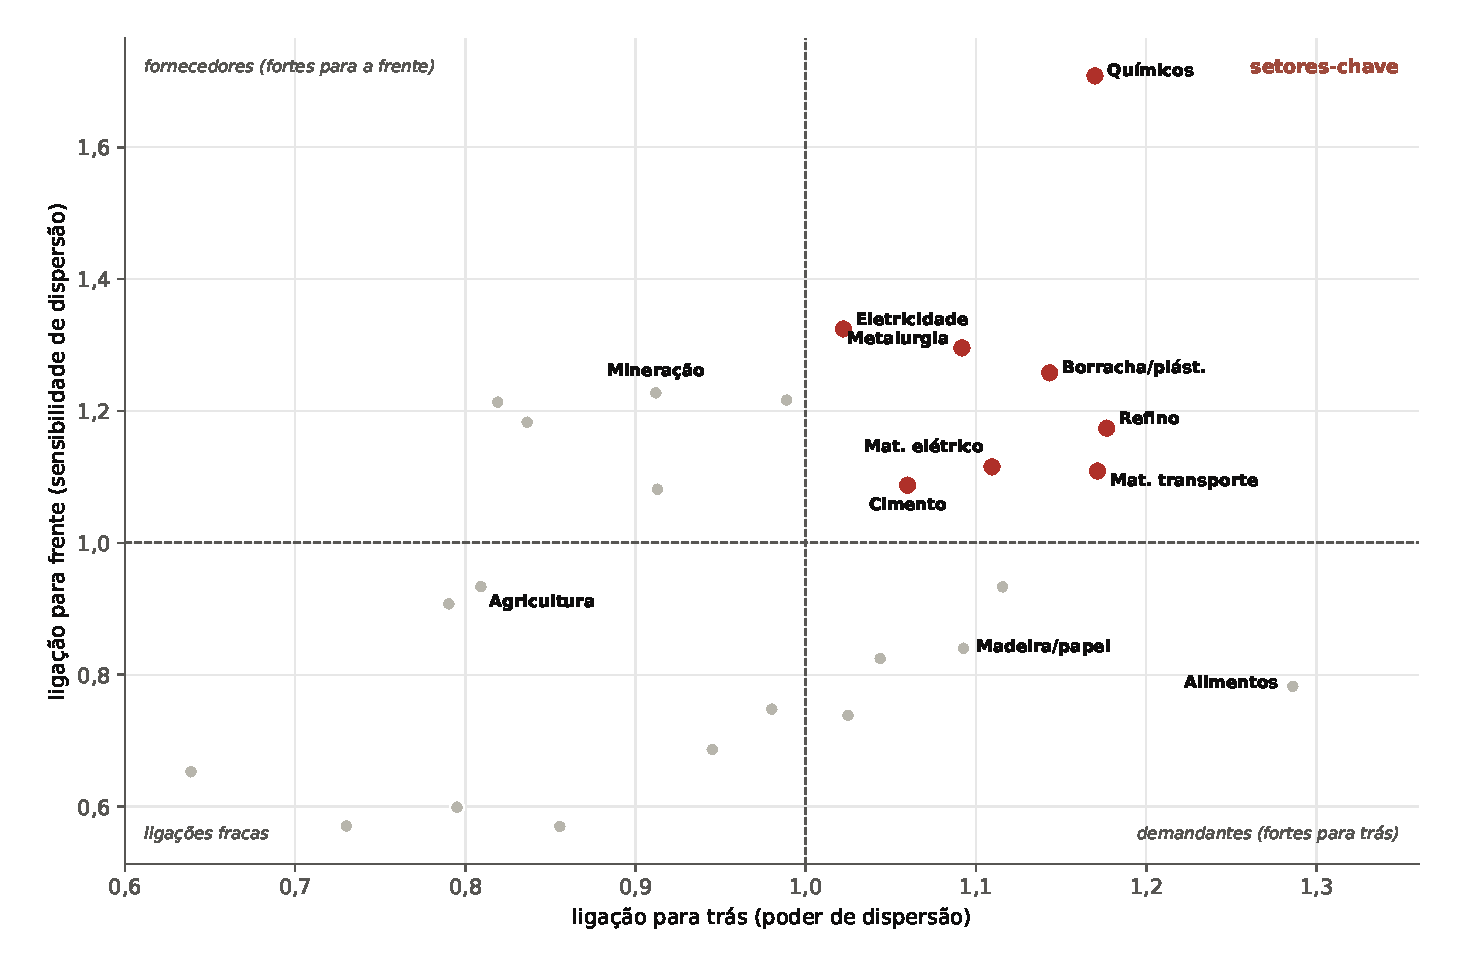
\includegraphics[width=.92\linewidth]{fig_setores_chave.pdf}
\fonte{Nota: o quadrante superior-direito (vermelho) reúne os setores-chave (poder e
sensibilidade de dispersão acima da média), todos rotulados; a mineração aparece como forte
fornecedora a montante, com baixa ligação para trás.\\
Fonte: elaboração própria a partir de
\href{https://github.com/fcarva/es-insumo-produto/blob/116a350/pesquisa/17_caracterizacao_es_2008.py}{\texttt{17\_caracterizacao\_es\_2008.py}}
(cálculo) e
\href{https://github.com/fcarva/es-insumo-produto/blob/116a350/pesquisa/19_fig_caracterizacao.py}{\texttt{19\_fig\_caracterizacao.py}}
(figura), sobre
\href{https://github.com/fcarva/es-insumo-produto/blob/116a350/pesquisa/outputs/es_caracterizacao_2008.csv}{\texttt{outputs/es\_caracterizacao\_2008.csv}}
\citep{carvalho2026repo}.}
\end{figure}

\paragraph{O ES é típico ou extremo? Um \emph{benchmark} interestadual.}
Que a extração tenha baixa ligação para trás é uma regularidade \emph{universal} ---
mineração e petróleo são pobres em insumos intermediários em qualquer economia. A pergunta
relevante não é \emph{se} o ES exibe a dualidade, mas se a exibe de forma \emph{distintiva}.
A comparação do ES com as 27 unidades da federação na matriz interestadual de 2008
(Tabela~\ref{tab:cluster}) dá uma resposta precisa: a dualidade é \textbf{genérica em tipo, mas
extrema em grau}.\footnote{Os valores do \emph{benchmark} interestadual são médias
\emph{ponderadas pela produção} sobre a matriz \emph{interestadual} (27 UFs), escolha que
garante comparabilidade entre estados; diferem, por isso, das médias \emph{simples} sobre a
matriz \emph{bi-regional} reportadas no início desta seção (produção 1,76; emprego 27,9). As
duas descrevem o mesmo fenômeno sob agregações distintas.} Nos indicadores neutros à
composição --- multiplicador de produção (1,66; 14\textordmasculine) e ligação para trás
ponderada (0,92; 14\textordmasculine) --- o ES é \emph{exatamente mediano}. É na
\emph{composição} e no \emph{emprego} que ele se destaca: é o \textbf{segundo} estado mais
intensivo em setores de base (36,4\%, só atrás de Mato Grosso)\footnote{A classificação
base/\emph{commodity}
(\href{https://github.com/fcarva/es-insumo-produto/blob/116a350/pesquisa/10_cluster_setorial.py}{\texttt{10\_cluster\_setorial.py}})
inclui Alimentos entre os setores de base --- escolha que eleva as parcelas de todos os
estados, sobretudo dos cinco do grupo dinâmico cujo setor dominante é Alimentos
(Tabela~\ref{tab:cluster}). O traço capixaba que independe desse rótulo é o setor
\emph{dominante}: o ES é um dos três únicos estados do país, com Pará e Rio de Janeiro,
liderados pela extrativa mineral. A reestimação do ranking excluindo Alimentos do rótulo fica
registrada como checagem de replicação sobre
\href{https://github.com/fcarva/es-insumo-produto/blob/116a350/pesquisa/22_benchmark_caracterizacao.py}{\texttt{22\_benchmark\_caracterizacao.py}}
e
\href{https://github.com/fcarva/es-insumo-produto/blob/116a350/pesquisa/10_cluster_setorial.py}{\texttt{10\_cluster\_setorial.py}}.}
e está entre os de \textbf{menor} multiplicador de emprego (25,4 empregos por R\$ milhão;
24\textordmasculine\ de 27). O sintoma mais nítido: o emprego gerado por seu setor dominante
equivale a apenas 39\% da média dos setores do estado --- o \textbf{segundo} valor mais baixo
do país (mediana 65\%). O Espírito Santo não é, pois, um contraexemplo da regularidade, mas um
de seus \emph{casos-limite}: a economia em que a base extrativa-industrial pesa mais e menos
emprego direto distribui.

% TODO EDITORIAL (A4): "estados de crescimento dinâmico" e o aposto "subcobertos pelo
% mercado de capitais" introduzem um critério externo que o artigo nunca define. Ou
% acrescentar uma frase de definição com a fonte do critério, ou trocar por um rótulo
% autoexplicativo. A comparação de razão de feedback da seção 7 (0,49%) depende dele.
A composição reforça o ponto (Tabela~\ref{tab:cluster}): entre os oito estados de crescimento
dinâmico --- subcobertos pelo mercado de capitais, excluído o núcleo SP/RJ ---, o ES é o mais
intensivo em mineração e o segundo em setores de base, com o menor multiplicador relativo de
emprego. É a composição, não a decomposição, que o singulariza. O paralelo mais próximo é
Minas Gerais, economia mineral vizinha cuja matriz bi-regional \citep{domingues2002matriz}
já documentava transbordamentos intensos, e pouco recíprocos, ao restante do país.

\begin{table}[tbp]
\caption{\emph{Benchmark} interestadual: o ES e os estados de crescimento dinâmico
\emph{versus} o núcleo SP/RJ e a mediana das 27 UFs (2008)}
\label{tab:cluster}
\centering\small
\setlength{\tabcolsep}{4.5pt}
\begin{threeparttable}
\begin{tabular}{lrrrrrl}
\toprule
Estado & PIB (\%) & Vazam.\ (\%) & Base (\%) & Mult.\ empr. & Líder$\div$média & Setor dominante\\
\midrule
\textbf{ES} & 2,2 & 22,8 & \textbf{36,4} & \textbf{25,4} & \textbf{0,39} & Mineração\\
MG & 9,5 & 20,9 & 29,6 & 30,9 & 0,47 & Metalurgia\\
SC & 4,1 & 22,5 & 21,7 & 30,6 & 1,29 & Alimentos\\
PR & 6,0 & 22,3 & 28,0 & 31,2 & 1,32 & Alimentos\\
RS & 6,7 & 21,8 & 24,6 & 30,3 & 1,37 & Alimentos\\
GO & 2,6 & 25,1 & 32,8 & 38,2 & 1,10 & Alimentos\\
MT & 1,8 & 27,4 & 43,4 & 40,2 & 1,37 & Agricultura\\
MS & 1,1 & 25,7 & 30,1 & 38,3 & 1,06 & Alimentos\\
\midrule
SP \emph{(núcleo)} & 32,0 & 14,2 & 18,0 & 24,0 & 1,46 & Serviços\\
RJ \emph{(núcleo)} & 11,2 & 15,6 & 27,4 & 22,4 & 0,47 & Mineração\\
\midrule
Mediana (27 UFs) & --- & --- & 21,0 & 42,5 & 0,65 & ---\\
\bottomrule
\end{tabular}
\begin{tablenotes}[flushleft]\footnotesize
\item Nota: ``Base'' é a participação dos setores de base/\emph{commodity} no VBP;
``Mult.\ empr.'' é o multiplicador de emprego ponderado (empregos por R\$\,1 milhão);
``Líder$\,\div\,$média'' é o emprego gerado pelo setor dominante em razão da média dos
setores do estado.
\item Nota: o ES é o 2\textordmasculine\ mais intensivo em setores de base, tem um dos menores
multiplicadores de emprego (24\textordmasculine\ de 27), o 2\textordmasculine\ menor emprego
relativo do líder e, com Pará e Rio de Janeiro, é um dos três estados do país cujo setor
dominante é a Mineração.
\item Fonte: elaboração própria a partir de
\href{https://github.com/fcarva/es-insumo-produto/blob/116a350/pesquisa/22_benchmark_caracterizacao.py}{\texttt{22\_benchmark\_caracterizacao.py}}
sobre
\href{https://github.com/fcarva/es-insumo-produto/blob/116a350/pesquisa/outputs/cluster_setorial.csv}{\texttt{outputs/cluster\_setorial.csv}}
\citep{carvalho2026repo}.
\end{tablenotes}
\end{threeparttable}
\end{table}

% =====================================================================
\section{O panorama temporal (2010--2021)}
\label{sec:panorama}
Uma ressalva de objeto antecede esta seção. O Espírito Santo dispõe apenas de \emph{âncoras}
insumo-produto --- 2008 (estadual) e 2015 (microrregional) ---, não de uma série anual própria.
O que a série nacional de 68 setores (2010--2021) oferece não é, portanto, a trajetória da
\emph{estrutura capixaba}, e sim o \textbf{pano de fundo nacional} dos setores que a definem:
como evoluiu, no país, a posição estrutural da extração, da siderurgia, do refino e da
celulose --- os ramos sobre os quais a economia do ES está montada. É uma leitura de tendência
\emph{dos setores}, não \emph{do estado}; lida nesses termos, ela é informativa
(Figura~\ref{fig:traj}). A leitura confirma, ao longo do tempo, a \emph{dualidade} do retrato
de 2008. O setor de \textbf{celulose e papel} é o mais consistente entre os setores-chave, e em
fortalecimento --- sua ligação para trás sobe de 1,41 (2010) para 1,51 (2021) e seu
multiplicador de produção, de 2,85 para 3,05. A \textbf{siderurgia} é setor-chave na maior
parte do período (ligação para trás entre 1,2 e 1,4), com um recuo em 2021 que merece cautela
interpretativa: a queda concentra-se na cadeia metálica (ferro-gusa, metais não ferrosos,
produtos de metal) e é coerente com o \emph{salto de preços do aço} em 2021, que incide sobre
matrizes a preços correntes --- quando o valor da produção sobe mais que as compras
intermediárias, o coeficiente técnico $a_{ij}=z_{ij}/x_j$ cai por efeito nominal, não por
desintegração estrutural. O \textbf{refino} mantém-se no limiar de setor-chave. Já a
\textbf{extração de petróleo e gás} e a \textbf{extração de minério de ferro} operam como
enclaves: suas ligações para trás permanecem \emph{abaixo da unidade} em quase todos os anos
--- compram poucos insumos domésticos ---, e o minério de ferro registra seu pico de
integração em 2015--2016, coincidindo com o rompimento da barragem de Fundão, e recua em
seguida. A transformação carrega os encadeamentos; a extração os dispensa.

\begin{figure}[tbp]
\centering
\caption{Ligação para trás dos setores de base do ES na estrutura nacional (2010--2021)}
\label{fig:traj}
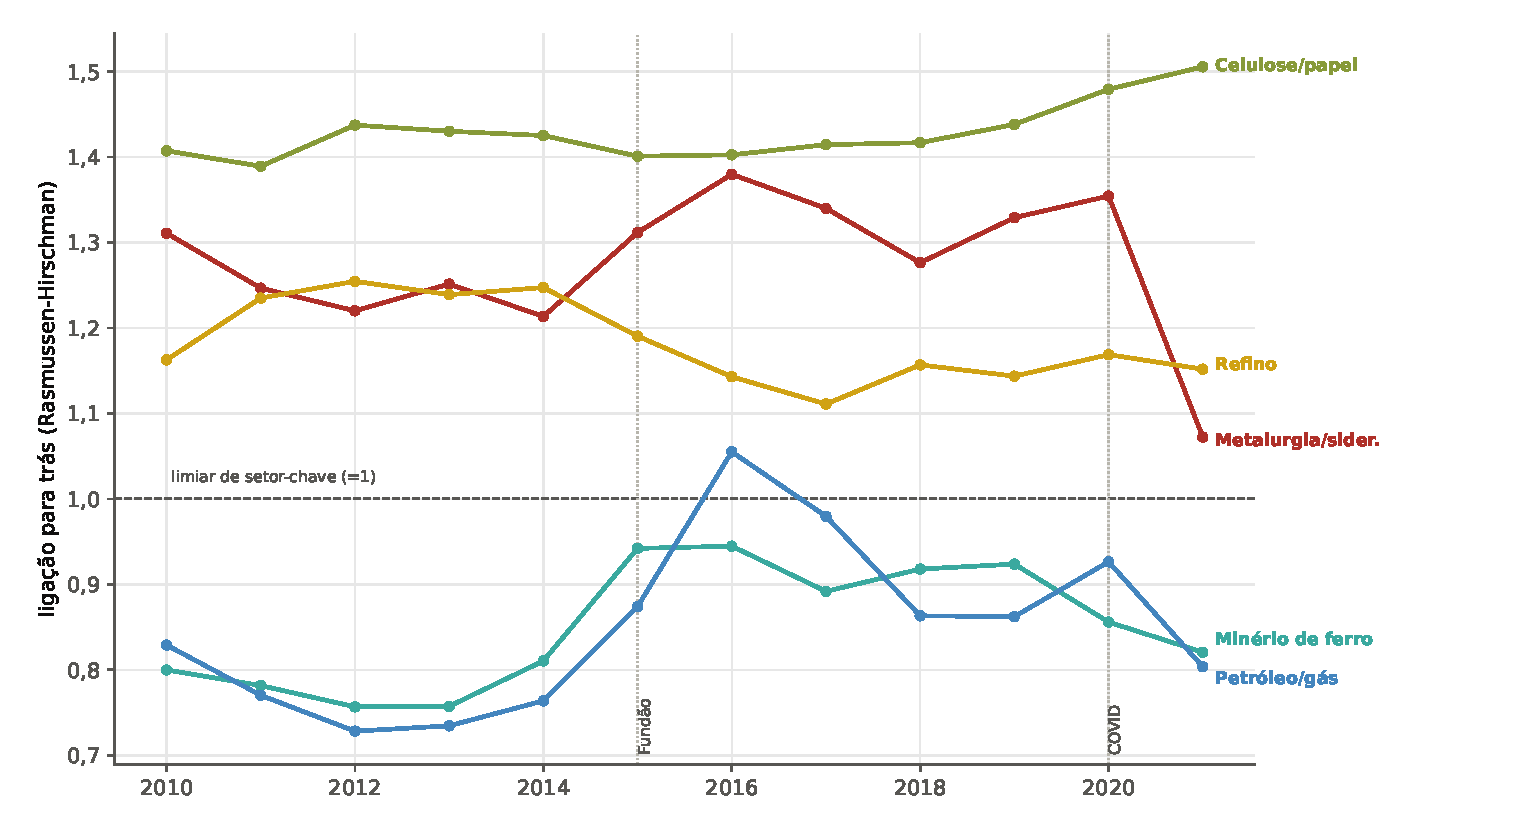
\includegraphics[width=.95\linewidth]{fig_trajetoria_n68.pdf}
\fonte{Nota: série de 68 setores. Celulose e siderurgia acima da unidade (setores-chave);
extração de petróleo e de minério abaixo (enclaves de baixa ligação doméstica).\\
Fonte: elaboração própria a partir de
\href{https://github.com/fcarva/es-insumo-produto/blob/116a350/pesquisa/18_trajetoria_n68.py}{\texttt{18\_trajetoria\_n68.py}}
(cálculo) e
\href{https://github.com/fcarva/es-insumo-produto/blob/116a350/pesquisa/19_fig_caracterizacao.py}{\texttt{19\_fig\_caracterizacao.py}}
(figura), sobre
\href{https://github.com/fcarva/es-insumo-produto/blob/116a350/pesquisa/outputs/trajetoria_n68.csv}{\texttt{outputs/trajetoria\_n68.csv}}
\citep{carvalho2026repo}.}
\end{figure}

% =====================================================================
\section{A composição territorial (2015)}
\label{sec:territorio}
O sistema das dez microrregiões revela um \emph{mosaico de especializações}
(Figura~\ref{fig:vocacao}). A Região Metropolitana (Grande Vitória) concentra 62\% da
produção estadual e é o núcleo diversificado --- petróleo, siderurgia (a usina de
Tubarão) e serviços. Ao seu redor dispõem-se territórios especializados, cada qual com um
quociente locacional elevado em seu setor: \textbf{celulose} no Rio Doce
($\mathrm{LQ}\,8{,}2$; corredor Linhares/Aracruz), \textbf{rochas ornamentais} no
Central Sul ($\mathrm{LQ}\,7{,}7$; Cachoeiro de Itapemirim), \textbf{minério de ferro e
pelotização} no Litoral Sul ($\mathrm{LQ}\,9{,}5$; Anchieta), \textbf{têxtil} no
Centro-Oeste ($\mathrm{LQ}\,9{,}6$; Colatina) e um interior \textbf{agropecuário} nas
serranas e no Caparaó --- com destaque para a pecuária/avicultura na Central Serrana
($\mathrm{LQ}\,21{,}9$; Santa Maria de Jetibá). A economia capixaba não é homogênea: é
um núcleo industrial-exportador cercado por especializações regionais nítidas.
Um padrão menos óbvio do que o do mapa de especialização emerge ao medir a
\emph{concentração} da composição setorial de cada microrregião (índice de Herfindahl): ela
não acompanha o porte (correlação $\approx0$), mas a \emph{composição} --- os territórios
extrativos (Litoral Sul, minério, HHI 0,18; Nordeste, petróleo, 0,14) são os mais
mono-estruturais, reproduzindo na escala territorial o mesmo padrão-\emph{enclave} que a
extração exibe na escala setorial, ao passo que o núcleo metropolitano é diversificado.

\paragraph{Multiplicadores e retenção territorial.}
A bateria de multiplicadores aplicada ao sistema microrregional (350$\times$350)
quantifica o desenho centro-periferia que o mapa de especialização sugere
(Tabela~\ref{tab:micro}). O multiplicador de produção \emph{simples} é praticamente
idêntico entre as dez microrregiões ($\approx$1,57--1,58) --- consequência esperada da
regionalização IIOAS, que aplica a mesma tecnologia nacional a todos os territórios; as
ligações de Rasmussen--Hirschman são, pela mesma razão, quase invariantes no espaço, de
modo que \emph{setores-chave} são um atributo da tecnologia, não do território. O que
diferencia os territórios é a \emph{composição} e, sobretudo, a \emph{retenção}: na média
ponderada pelo porte setorial, o multiplicador vai de 1,42 (Caparaó) a 1,76 (Litoral Sul,
inflado pela pelotização), mas a parcela dele que se realiza \emph{dentro} da própria
microrregião varia de \textbf{90,9\%} na Metropolitana a \textbf{66,2\%} no Litoral Sul
extrativo --- a periferia compra seus insumos na metrópole, não em si mesma. É a mesma
assinatura de enclave, agora na dimensão territorial do fluxo. A \emph{extração hipotética}
\citep{dietzenbacher1993} fecha o desenho: removida a Metropolitana do sistema, a produção
das demais microrregiões cairia \textbf{13,0\%} --- a periferia capixaba depende do núcleo
capixaba como o estado, visto de fora, depende do Sudeste (\S\ref{sec:plataforma}).

\begin{table}[tbp]
\caption{Multiplicadores de produção e renda e retenção intra-territorial do multiplicador,
por microrregião (2015)}
\label{tab:micro}
\centering\small
\begin{threeparttable}
\begin{tabular}{lrrrr}
\toprule
Microrregião & \% do VBP do ES & Mult.\ produção (pond.) & Retenção intra (\%) & Mult.\ renda \\
\midrule
Metropolitana & 62,3 & 1,64 & 90,9 & 0,37 \\
Rio Doce & 10,6 & 1,64 & 74,3 & 0,31 \\
Central Sul & 6,2 & 1,60 & 79,4 & 0,38 \\
Nordeste & 4,9 & 1,50 & 85,3 & 0,32 \\
Centro-Oeste & 4,4 & 1,53 & 85,6 & 0,38 \\
Litoral Sul & 4,1 & 1,76 & 66,2 & 0,34 \\
Noroeste & 2,1 & 1,50 & 87,3 & 0,36 \\
Caparaó & 1,9 & 1,42 & 88,2 & 0,39 \\
Sudoeste Serrana & 1,9 & 1,48 & 80,6 & 0,37 \\
Central Serrana & 1,5 & 1,43 & 82,3 & 0,31 \\
\bottomrule
\end{tabular}
\begin{tablenotes}[flushleft]\footnotesize
\item Nota: multiplicadores de tipo I, ponderados pelo VBP setorial. A metrópole retém; a
periferia extrativa vaza.
\item Nota: a retenção é a razão das somas ponderadas
($\sum_j w_j O^{\mathrm{intra}}_j / \sum_j w_j O_j$) e difere, por construção, da média
ponderada das razões setoriais usada em \S\ref{sec:plataforma} e no Apêndice~\ref{ap:s23}
(Metropolitana: vazamento de 8,4\%, i.e., retenção de 91,6\%); as duas agregações descrevem o
mesmo fluxo.
\item Fonte: elaboração própria a partir de
\href{https://github.com/fcarva/es-insumo-produto/blob/116a350/pesquisa/24_micro_mult_chave.py}{\texttt{24\_micro\_mult\_chave.py}}
sobre
\href{https://github.com/fcarva/es-insumo-produto/blob/116a350/pesquisa/outputs/micro_multiplicadores.csv}{\texttt{outputs/micro\_multiplicadores.csv}}
\citep{carvalho2026repo}.
\end{tablenotes}
\end{threeparttable}
\end{table}

Esta leitura dialoga com \citet{ribeiro2024dinamica}, que regionalizaram a mesma matriz de
2015 e identificaram setores-chave por microrregião --- alimentos, eletricidade, minerais
não metálicos --- pela geração de emprego e renda. O quociente locacional e a retenção
acrescentam a esse retrato as dimensões da \emph{especialização} e do \emph{fluxo}: não
apenas onde os multiplicadores são altos, mas em que cada território é especializado e
quanto do encadeamento fica nele. Os dois resultados convergem para o mesmo desenho --- um
estado polarizado entre núcleo e periferias especializadas.

\begin{figure}[tbp]
\centering
\caption{Quociente locacional por setor e microrregião (2015)}
\label{fig:vocacao}
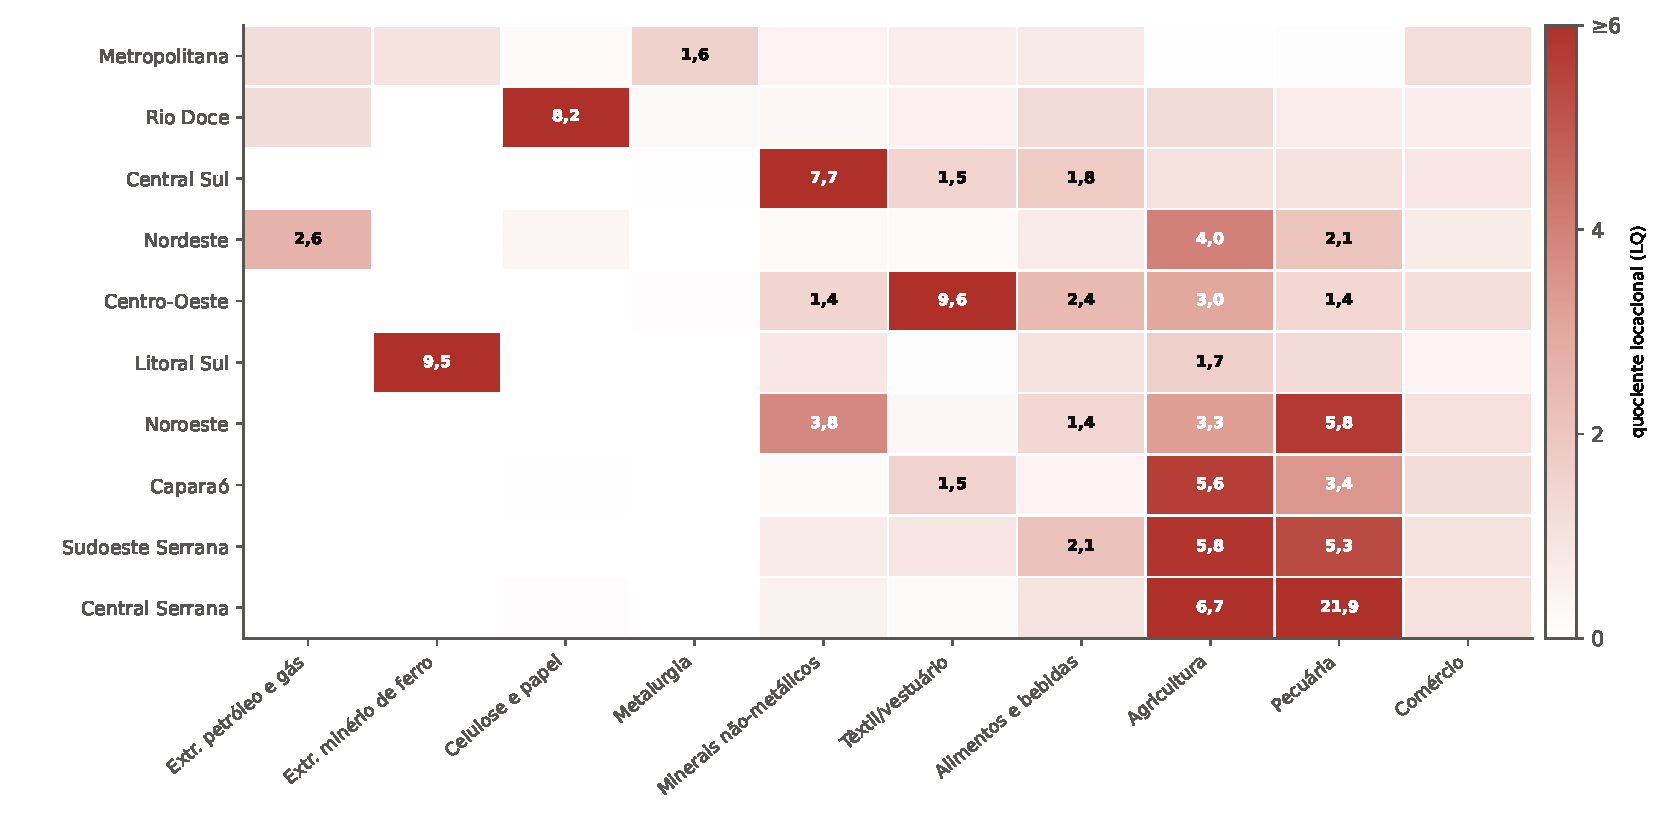
\includegraphics[width=\linewidth]{fig_micro_vocacao.pdf}
\fonte{Nota: cada território concentra (vermelho) o setor de sua composição; a Metropolitana,
diversificada, não exibe especialização extrema. Exibem-se os dez setores (de 35) que definem
as especializações territoriais; a escala de cor é truncada em $\mathrm{LQ}=6$ --- os valores
anotados são os exatos.\\
Fonte: elaboração própria a partir de
\href{https://github.com/fcarva/es-insumo-produto/blob/116a350/pesquisa/20_caracterizacao_micro.py}{\texttt{20\_caracterizacao\_micro.py}}
(cálculo) e
\href{https://github.com/fcarva/es-insumo-produto/blob/116a350/pesquisa/21_fig_micro.py}{\texttt{21\_fig\_micro.py}}
(figura), sobre
\href{https://github.com/fcarva/es-insumo-produto/blob/116a350/pesquisa/outputs/micro_LQ.csv}{\texttt{outputs/micro\_LQ.csv}}
\citep{carvalho2026repo}.}
\end{figure}

% =====================================================================
\section{Abertura, vazamento e a face plataforma}
\label{sec:plataforma}
Caracterizada a estrutura --- setorial, temporal e territorial ---, resta a dimensão que a
\emph{conecta} ao resto do país: a abertura. Aqui a economia de base revela-se também uma
\emph{economia-plataforma}, no sentido de que seu encadeamento se realiza, em boa parte, fora
do estado.

\paragraph{Vazamento.} Em média, \textbf{24,9\%} do multiplicador de produção capixaba vaza
para fora do ES (22,9\% na média ponderada pela produção) --- número convergente, em safra e
agregação distintas, com os 27,4\% de \citet{haddad2017iioas}. A distribuição setorial completa
está na Tabela~\ref{tab:setores}: serviços imobiliários quase não vazam (5,2\%), enquanto
alimentos vazam 37,4\%. No emprego, o vazamento dos setores
pesados é ainda maior --- metade ou mais do trabalho que a demanda capixaba mobiliza realiza-se
fora do estado: refino 61,6\%, alimentos 56,5\%, madeira/papel 50,3\% e metalurgia 49,3\%.

\begin{table}[tbp]
\caption{Multiplicador de produção, vazamentos de produção e de emprego e ligações de
Rasmussen--Hirschman dos 26 setores do ES (2008)}
\label{tab:setores}
\centering\small
\begin{threeparttable}
\begin{tabular}{lrrrrr}
\toprule
Setor & $O_j$ & Vaz.\ prod.\ (\%) & Vaz.\ empr.\ (\%) & Lig.\ trás & Lig.\ frente\\
\midrule
Imobiliário/aluguel & 1,15 & 5,2 & 12,3 & 0,64 & 0,65\\
Educação & 1,31 & 11,6 & 7,1 & 0,73 & 0,57\\
Financeiro/seguros & 1,47 & 12,8 & 20,6 & 0,82 & 1,21\\
Adm. pública & 1,43 & 15,0 & 16,0 & 0,80 & 0,60\\
Comércio & 1,42 & 16,0 & 7,6 & 0,79 & 0,91\\
Serviços privados & 1,50 & 17,9 & 8,4 & 0,84 & 1,18\\
Saúde & 1,54 & 19,1 & 14,9 & 0,86 & 0,57\\
Eletricidade/gás/água & 1,83 & 21,0 & 28,4 & 1,02 & 1,32\\
Agricultura/silvicultura & 1,45 & 21,6 & 9,9 & 0,81 & 0,93\\
Mineração & 1,64 & 22,7 & 42,4 & 0,91 & 1,23\\
Máquinas/equip. & 2,00 & 24,9 & 26,5 & 1,12 & 0,93\\
Construção & 1,70 & 25,5 & 16,1 & 0,95 & 0,69\\
Material de transporte & 2,10 & 26,1 & 29,7 & 1,17 & 1,11\\
Refino/coque/álcool & 2,11 & 27,8 & 61,6 & 1,18 & 1,17\\
Têxtil/vestuário & 1,87 & 28,1 & 17,8 & 1,04 & 0,82\\
Metalurgia & 1,96 & 29,2 & 49,2 & 1,09 & 1,30\\
Químicos/farmacêuticos & 2,10 & 29,4 & 41,2 & 1,17 & 1,71\\
Mat. elétrico/eletrônicos & 1,99 & 29,8 & 34,1 & 1,11 & 1,12\\
Pecuária e pesca & 1,64 & 30,2 & 19,4 & 0,91 & 1,08\\
Transporte/armazenagem & 1,77 & 30,3 & 23,1 & 0,99 & 1,22\\
Indústrias diversas & 1,84 & 30,5 & 16,3 & 1,02 & 0,74\\
Min. não-metálicos & 1,90 & 30,6 & 28,2 & 1,06 & 1,09\\
Alojamento/alimentação & 1,76 & 31,9 & 22,2 & 0,98 & 0,75\\
Madeira/papel & 1,96 & 35,8 & 50,3 & 1,09 & 0,84\\
Borracha/plástico & 2,05 & 36,8 & 32,9 & 1,14 & 1,26\\
Alimentos/bebidas/fumo & 2,31 & 37,4 & 56,5 & 1,29 & 0,78\\
\midrule
\textbf{Média (simples)} & 1,76 & 24,9 & 26,6 & 0,98 & 0,99\\
\textbf{Média (ponderada)} & 1,66 & 22,9 & 26,0 & 0,92 & 1,01\\
\bottomrule
\end{tabular}

\begin{tablenotes}[flushleft]\footnotesize
\item Nota: setores ordenados pelo vazamento do multiplicador de produção. Vazamento médio:
simples 24,9\%; ponderado pela produção 22,9\%.
\item Fonte: elaboração própria a partir de
\href{https://github.com/fcarva/es-insumo-produto/blob/116a350/pesquisa/12_tab_setores.py}{\texttt{12\_tab\_setores.py}}
sobre
\href{https://github.com/fcarva/es-insumo-produto/blob/116a350/pesquisa/outputs/es_setores_resultados.csv}{\texttt{outputs/es\_setores\_resultados.csv}}
\citep{carvalho2026repo}.
\end{tablenotes}
\end{threeparttable}
\end{table}

\paragraph{\emph{Spillover} e \emph{feedback}.} Uma injeção de R\$\,51,5 bilhões na demanda
final do ES por produtos do ES transborda R\$\,18,2 bilhões de produção para o restante do país
(35\% da injeção), mas o \emph{feedback} de volta é de apenas R\$\,164 milhões ---
\textbf{0,32\%} (Figura~\ref{fig:sankey}). A interdependência é quase unilateral. O destino,
além disso, é concentrado: o \textbf{Sudeste} (excluído o ES) absorve \textbf{65,4\%} do
\emph{spillover} --- São Paulo 37,8\%, Rio de Janeiro 14,7\% e Minas Gerais 12,9\% --- e o
núcleo São Paulo--Rio de Janeiro, \textbf{52,5\%}. O ES alimenta seus vizinhos mais ricos; o
encadeamento que escapa é capturado a jusante e quase não retorna. O padrão não é
exclusividade capixaba entre os estados exportadores de \emph{commodities}: em Mato Grosso, a
soja gera 8 empregos diretos por R\$\,1 milhão de demanda final, ante 31 indiretos
\citep{figueiredo2004agriculture}; no agronegócio gaúcho, \citet{peixoto2013metodologia}
estimam que apenas 0,4\% do valor adicionado do restante do Brasil decorre de elos com o Rio
Grande do Sul, ante 7,9\% no sentido inverso --- a mesma assimetria de captura a jusante que o
ES exibe pelo lado do minério.

\begin{figure}[tbp]
\centering
\caption{Destino do \emph{spillover} do ES, estratificado por macrorregião e estado (2008)}
\label{fig:sankey}
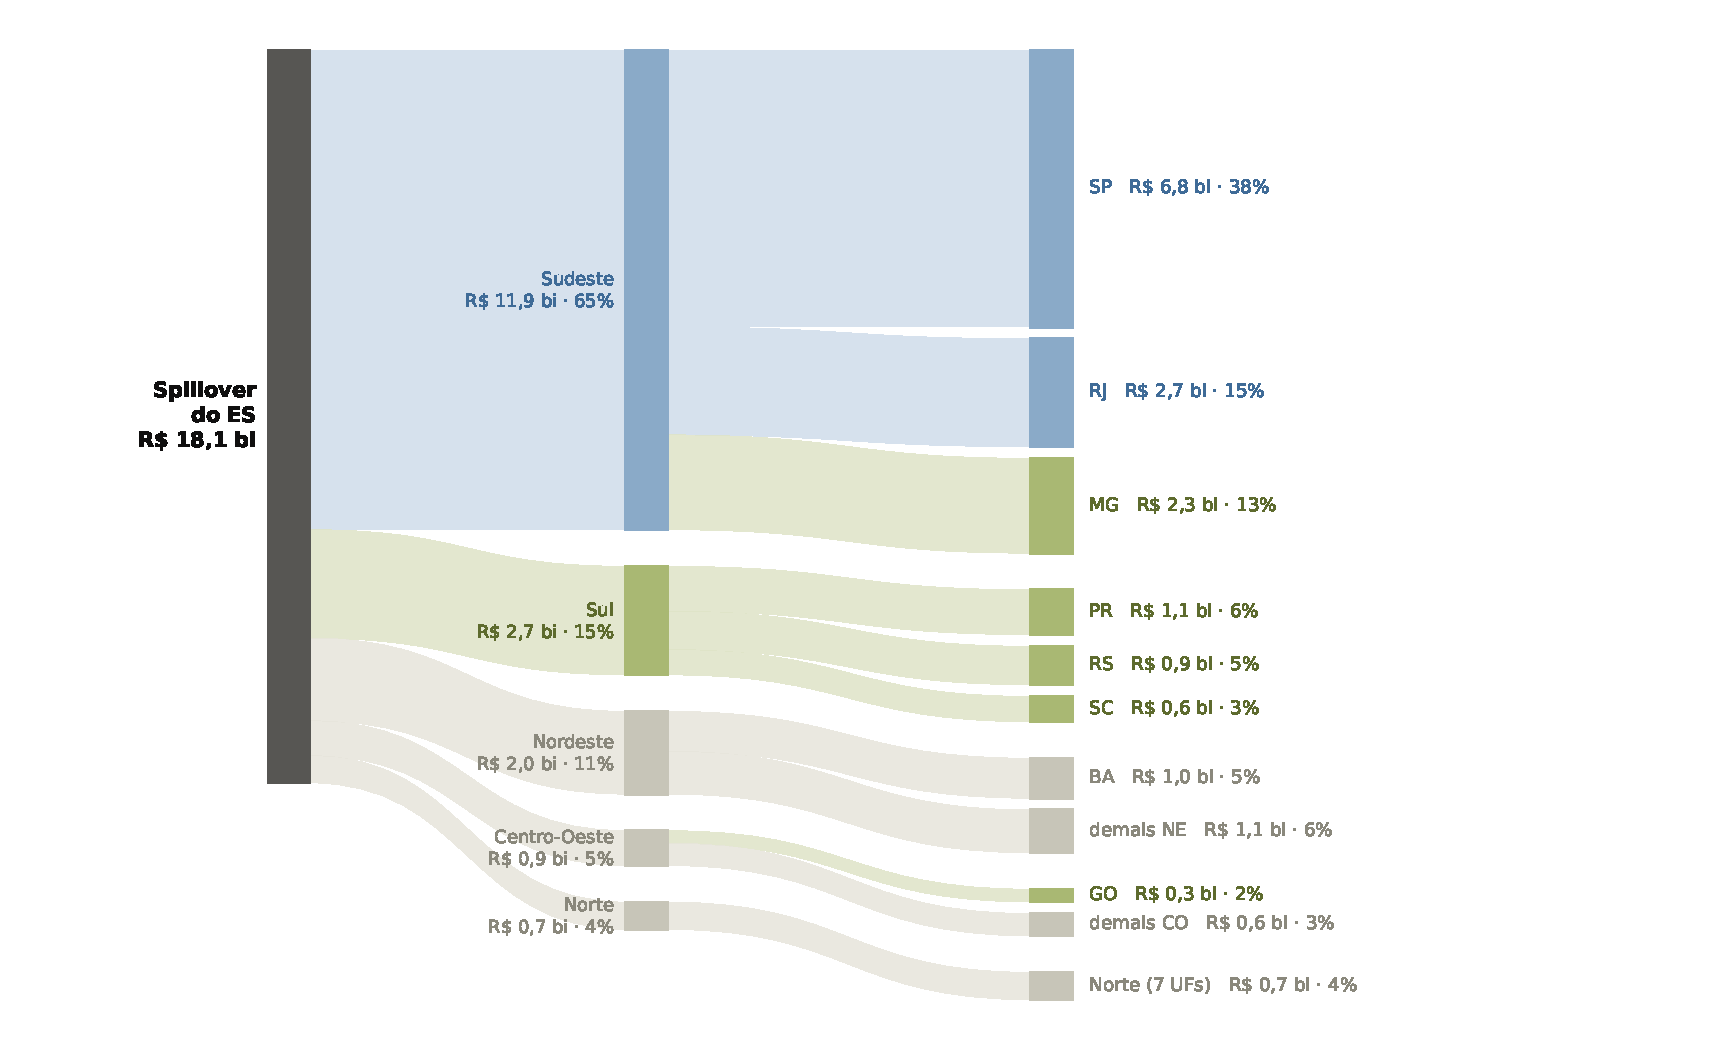
\includegraphics[width=.92\linewidth]{es_sankey.pdf}
\fonte{Nota: injeção da demanda final do ES por produtos do ES, matriz interestadual de 2008.
Dos R\$\,18,1 bilhões transbordados, o Sudeste absorve 65\% e o núcleo São Paulo--Rio de
Janeiro, 52,5\%; o \emph{feedback} de volta ao ES é de apenas 0,32\% da injeção. No sistema
bi-regional do texto, o mesmo experimento transborda R\$\,18,2 bi --- a diferença é de
agregação (Apêndice~\ref{ap:medias}).\\
Fonte: elaboração própria a partir de
\href{https://github.com/fcarva/es-insumo-produto/blob/116a350/pesquisa/02_interestadual.py}{\texttt{02\_interestadual.py}}
(cálculo) e
\href{https://github.com/fcarva/es-insumo-produto/blob/116a350/pesquisa/11_fig_sankey.py}{\texttt{11\_fig\_sankey.py}}
(figura), sobre
\href{https://github.com/fcarva/es-insumo-produto/blob/116a350/pesquisa/outputs/es_spillover_destino.csv}{\texttt{outputs/es\_spillover\_destino.csv}}
\citep{carvalho2026repo}.}
\end{figure}

\paragraph{Escalas aninhadas.} Essa lógica-plataforma não é exclusiva da relação entre o ES e o
Brasil --- ela \emph{se reproduz dentro} do estado. A Região Metropolitana retém o multiplicador
(vazamento de 8,4\%, 62\% da produção estadual), enquanto a periferia primário-exportadora vaza
encadeamento \emph{para a metrópole} (até 76\% de seu \emph{spillover}). O par
retenção-no-núcleo / vazamento-na-periferia configura, pois, a relação \emph{centro-periferia}
das três lentes da \S\ref{sec:quadro}, reproduzida em \emph{escalas aninhadas}: a periferia
está para o ES como o ES está para o Sudeste --- reproduz-se, dentro do estado, o mesmo desenho
que a tradição regional brasileira lê entre o ES e o núcleo industrial paulista. É a mesma
assinatura de \emph{enclave} que a concentração territorial já indicava
(\S\ref{sec:territorio}), agora pelo lado do fluxo. A pequenez do \emph{feedback}, por sua vez,
é regularidade conhecida desde \citet{miller1966} e, nos dados de 2008, privilégio de núcleo: a
razão de \emph{feedback} média de SP+RJ (1,97\%) é quatro vezes a dos oito estados de
crescimento dinâmico (0,49\%). Nem a concentração do destino singulariza o ES --- Minas Gerais
(60,0\%) e Rio Grande do Sul (55,2\%) escoam ao núcleo parcela \emph{maior} que a capixaba
(52,5\%). O que é próprio do ES, como mostra o \emph{benchmark} composicional
(Tabela~\ref{tab:cluster}), não é a mecânica do vazamento, mas a \emph{composição de base}
que essa mecânica genérica transporta.

% =====================================================================
\section{Discussão}
\label{sec:discussao}
O conjunto desenha o ES como uma \textbf{economia de base, dual e pouco geradora de
trabalho direto em seus setores líderes}. Esse perfil dialoga com o debate
brasileiro sobre \emph{desindustrialização} e \emph{primarização} da estrutura produtiva ---
debate que a literatura nacional de insumo-produto examinou com as \emph{mesmas} ferramentas
aqui empregadas. \citet{morceiro2012} documenta, por índices de ligação de
Rasmussen--Hirschman e indicadores de conteúdo importado, a erosão dos encadeamentos da
indústria brasileira; já \citet{nassif2015}, pelos índices de ligação entre 1996 e 2009,
relativizam a tese e encontram pouca evidência de desindustrialização agregada --- no plano
nacional, o debate permanece em aberto. A contribuição do caso capixaba não é arbitrá-lo, mas
mostrar, na escala estadual, uma economia já estruturalmente \emph{especializada em setores de
base}: o ES exibe de forma concentrada o perfil de baixa ligação doméstica e baixa geração de
emprego que a literatura de desindustrialização \citep{oreiro2010} e de doença holandesa
\citep{cordenneary1982} associa às economias intensivas em recursos --- e o \emph{benchmark}
confirma que o faz de modo particularmente agudo. Os setores que a definem --- mineração,
petróleo, siderurgia, celulose --- têm grande porte, alta ligação para frente e os
maiores polos de crescimento pela medida de ligações puras; mas é a sua condição de
fornecedores a montante, e não de articuladores a jusante, que se destaca. A
consequência distributiva é direta: o emprego e a renda diretos vêm de outros setores
(intensivos em trabalho e serviços), de modo que o dinamismo da base não se traduz
automaticamente em ocupação --- a decomposição da demanda final dá a medida exata desse
descolamento: a demanda externa puxa 61,7\% da produção, mas 47,5\% do emprego
(Tabela~\ref{tab:decomp}). A essa fragilidade setorial soma-se uma fragilidade
\emph{geográfica}: como mostra a face plataforma (\S\ref{sec:plataforma}), o encadeamento que
a base gera \emph{vaza} para o núcleo SP--RJ com retorno quase nulo --- a captura de valor não
é só um problema de \emph{composição} setorial, mas também de \emph{posição} na hierarquia
regional, e essa lógica repete-se, em escala aninhada, da periferia capixaba para a Grande
Vitória. Base exportadora que comanda a produção, polos motrizes que concentram o encadeamento
e hierarquia centro-periferia que captura o valor são, aqui, três descrições de um mesmo dado
--- as três lentes da \S\ref{sec:quadro} convergindo sobre o mesmo sistema.
A dualidade entre extração-enclave e
transformação-chave, visível no retrato de 2008 e persistente na série 2010--2021,
admitiria uma leitura prescritiva --- adensar a jusante da cadeia
minério\,$\to$\,aço\,$\to$\,produtos de metal, cujos elos intermediários já são
setores-chave; eleger a celulose como prioridade, único setor de base cuja ligação para trás
\emph{cresce} na série nacional (1,41\,$\to$\,1,51); diversificar cada território a partir de
sua especialização. Este artigo abstém-se dela. O que os indicadores caracterizam não é uma
carteira de apostas setoriais, e sim um \textbf{problema estrutural} --- e a tradição do
desenvolvimento regional brasileiro extrai, do mesmo tipo de dado, conclusões distintas
das de um receituário setorial. Na leitura de \citet{cano1985}, estendida em
\citet{cano2008desconcentracao}, a especialização de uma periferia não é falha de política
local corrigível por seleção de setores: é o modo como o território se integra à
acumulação comandada pelo núcleo. O caso capixaba é paradigmático dessa leitura --- a
industrialização de base foi decidida de fora, pelos grandes projetos
federais-exportadores dos anos 1970--80, que instalaram no estado a ponta \emph{a
montante} de cadeias cujos elos a jusante permaneceram no núcleo ou no exterior
\citep{macedo2002integracao}. Sob essa ótica, os números deste artigo --- ligações puras
concentradas na base (4,4 e 3,4), 65\% do \emph{spillover} absorvido pelo Sudeste com
\emph{feedback} de 0,32\%, retenção de 90,9\% no núcleo metropolitano contra 66,2\% na
periferia extrativa, queda de 13,0\% da produção periférica sem a metrópole --- não medem
oportunidades de adensamento à espera de política: medem a mecânica que torna o
adensamento localmente improvável enquanto a posição do estado na hierarquia
núcleo-periferia não mudar. O encadeamento a jusante da base capixaba existe; apenas se
realiza em outro lugar --- e a trajetória favorável da celulose é o dado de um setor, não
a refutação do desenho. \citet{cacador2009olhar} chegam, pela via dos indicadores de
inovação, a uma caracterização convergente para o período recente: uma economia que cresce
acima da média nacional e permanece periférica em sua base científico-tecnológica ---
crescimento sem a mudança estrutural correspondente.
% TODO EDITORIAL (A5): o trecho abaixo afirma que as participações governamentais são "o
% principal canal" de fixação de riqueza, sem que o artigo apresente qualquer dado fiscal —
% e a seção 8 declara que implicações de política ficam como inferências condicionais.
% Ou suavizar ("um canal decisivo") ou acrescentar a referência que sustenta a afirmação.
% Além disso, royalties aparecem só aqui: vale sinalizar o tema antes.
É esse quadro que dá aos
\textbf{royalties} o seu estatuto analítico: numa economia cujos setores líderes pouco
empregam (o ES tem o segundo menor emprego relativo do setor líder no país;
Tabela~\ref{tab:cluster})
e cujo retorno via encadeamento é quase nulo (\emph{feedback} de 0,32\%), a captura de
valor não se dá pelo circuito interindustrial, mas pelo circuito fiscal --- dado o peso do
petróleo (cerca de um quarto do produto estadual), as participações governamentais são o
principal canal pelo qual a riqueza que transita pelo território nele se fixa. Não se
trata de recomendação, e sim de caracterização: é a estrutura, não a ausência de aposta
setorial, que faz da via fiscal o canal de retorno que resta.

Fica registrada, por fim, a extensão \emph{ambiental} do diagnóstico: assim como escoa ao
núcleo o encadeamento que gera, a economia de base capixaba exporta \emph{carbono incorporado}
--- minério, siderurgia, refino e celulose são intensivos em CO$_2$. Estimar esse
\emph{carbono-plataforma} (multiplicador de emissão, vazamento de carbono e pegada da pauta
exportadora) é a agenda imediata, viável com o satélite de CO$_2$ da matriz interestadual de
2019 \citep{haddad2025matriz}, na linha de \citet{carvalho2009avaliacao}; o aparato
reprodutível já está montado, à espera do vetor de emissões.

% =====================================================================
\section{Limitações}
\label{sec:limites}
Cinco limites são declarados. \textbf{(i)} O panorama temporal cobre 2010--2021, o
horizonte da série insumo-produto; a leitura estrutural não alcança 2022--2025, que
exigiria indicadores não insumo-produto (Contas Regionais, comércio exterior, produção
de petróleo). \textbf{(ii)} A série de 68 setores é \emph{nacional}: a trajetória dos
setores de base é uma aproximação da tendência capixaba via composição da pauta, não a
estrutura do ES ano a ano --- o estado dispõe apenas das âncoras de 2008 e 2015. Ademais,
as matrizes da série estão a \emph{preços correntes} (sem deflação), de modo que oscilações
anuais em setores sensíveis a preço --- como o recuo da siderurgia em 2021, no auge do preço
do aço --- devem ser lidas como efeito nominal/relativo, não necessariamente estrutural.
\textbf{(iii)} Os fluxos inter-regionais e sub-estaduais são \emph{estimados} pelo
método IIOAS, e o sistema microrregional apresenta um setor com coeficientes
desbalanceados (informação; sensibilidade no Apêndice~\ref{ap:s23}), além de não trazer
vetor de emprego (apenas remunerações). Como em toda a família de métodos não censitários, os
fluxos origem-destino são aproximações --- métodos gravitacionais reproduzem melhor os fluxos
observados que os quocientes \citep{riddington2006comparison} e os coeficientes regionais
são sensíveis à calibragem \citep{flegg2016evaluating} ---, de modo que os percentuais
inter-regionais devem ser lidos como ordens de grandeza; a assimetria qualitativa do
\emph{feedback}, contudo, é invariante à convenção (Apêndice~\ref{ap:convencao}).
\textbf{(iv)} As ligações puras, por ponderarem pelo tamanho, favorecem setores
grandes; por isso são reportadas em conjunto com os índices de Rasmussen--Hirschman,
neutros em relação ao porte. \textbf{(v)} A leitura de ``economia-plataforma'' é uma
interpretação estrutural derivada dos multiplicadores, do \emph{spillover}/\emph{feedback} e do
\emph{benchmark} interestadual; não deve ser lida como tipologia causal universal.
% TODO EDITORIAL (A7): a frase seguinte descrevia o processo de revisão ("A auditoria desta
% versão separou os claims..."), não o artigo, e usava dois anglicismos. Reescrita abaixo;
% confirmar se convém mantê-la.
Distinguem-se, ao longo do texto, os resultados diretamente derivados das matrizes, as
aproximações obtidas de séries nacionais e as implicações de política --- estas últimas
mantidas como inferências condicionais.

% =====================================================================
\section{Conclusão}
\label{sec:conclusao}
A análise insumo-produto caracteriza o Espírito Santo como uma economia de base, a
montante e intensiva em recursos, \emph{puxada de fora} --- 61,7\% de sua produção é
induzida por demanda externa ao estado ---, cujos setores líderes geram muito encadeamento mas
pouco emprego e pouca renda diretos, e cuja estrutura é dual --- extração-enclave de um lado,
transformação-chave de outro. Ao longo de 2010--2021, a celulose se fortalece, a
siderurgia oscila e a extração permanece pouco integrada; no território, o estado é um
mosaico de especializações em torno de um núcleo metropolitano diversificado. O retrato, além
de sistemático e reprodutível, oferece o substrato quantitativo para o debate sobre
diversificação, adensamento de cadeia e captura de valor na economia capixaba.

% =====================================================================
\appendix
\section{Formulário metodológico}
\label{ap:metodologia}
Este apêndice reúne, equação a equação, o ferramental cujos resultados o corpo do texto
reporta. A notação segue \citet{millerblair2009}; todos os instrumentos estão implementados
nas rotinas reprodutíveis do repositório \citep{carvalho2026repo}. Em todo o apêndice supõe-se
$A\ge 0$ \emph{produtiva} (condição de Hawkins--Simon; raio espectral menor que a unidade), o
que garante que as inversas de Leontief utilizadas existem e são não negativas --- condição
verificada empiricamente em cada sistema (inversa não negativa e finita; a exceção de
coluna do sistema microrregional é documentada no Apêndice~\ref{ap:s23}).

\subsection{Sistema de Leontief e multiplicadores}
\label{ap:leontief}
Com $Z$ a matriz de fluxos intermediários e $x$ o vetor de produção, os coeficientes técnicos
são $A=Z\hat{x}^{-1}$ e o sistema de quantidades é
\begin{equation}
x=(I-A)^{-1}y \equiv By,
\label{eq:leontief}
\end{equation}
com $y$ a demanda final. O multiplicador de produção do setor $j$ é $O_j=\sum_i b_{ij}$; os de
emprego e renda são $E_j=\sum_i w_i\,b_{ij}$ e $R_j=\sum_i v_i\,b_{ij}$, com coeficientes
diretos $w_i=\mathrm{ocup}_i/x_i$ e $v_i=\mathrm{rem}_i/x_i$. No fechamento de
\emph{tipo II}, o modelo é aumentado com o setor-família do ES:
\begin{equation}
\bar{A}=\begin{bmatrix} A & h\\ v' & 0\end{bmatrix},
\qquad h_i=\frac{c_i}{\sum_{k\in L}\mathrm{rem}_k},
\label{eq:tipo2}
\end{equation}
em que $c_i$ é o consumo das famílias capixabas do produto $i$, o denominador é a renda
total das remunerações dos setores do ES ($L$) e $v$ é o vetor de coeficientes de renda
com $v_i=0$ para $i\notin L$; os multiplicadores de tipo II são computados sobre
$(I-\bar{A})^{-1}$, descartada a linha-família. Num sistema bi-regional, esse fechamento
fornece um \emph{limite inferior} do efeito induzido local: fechar também para o consumo
em produtos do restante do Brasil apenas \emph{acrescentaria} coeficientes não negativos
a $\bar{A}$, e a inversa de Leontief é monótona no coeficiente --- $A\le A'$ elemento a
elemento implica $(I-A)^{-1}\le(I-A')^{-1}$, pela série de Neumann.

\subsection{Partição inter-regional de Isard}
\label{ap:isard}
Sejam $L$ a região-foco e $M$ o resto do sistema. A matriz de coeficientes e a inversa de
Leontief particionam-se em blocos intra e inter-regionais \citep{isard1951,millerblair2009}:
\begin{equation}
A=\begin{bmatrix} A^{LL} & A^{LM}\\ A^{ML} & A^{MM}\end{bmatrix},
\qquad
\begin{bmatrix} x^{L}\\ x^{M}\end{bmatrix}
=\begin{bmatrix} B^{LL} & B^{LM}\\ B^{ML} & B^{MM}\end{bmatrix}
\begin{bmatrix} y^{L}\\ y^{M}\end{bmatrix}.
\label{eq:isard}
\end{equation}
No caso geral, $x^{L}=B^{LL}y^{L}+B^{LM}y^{M}$. Para uma injeção restrita à demanda por
produtos de $L$ ($y^{M}=0$ --- o experimento de \S\ref{sec:plataforma}), resolver para $L$
dá a forma reduzida com o termo de \emph{feedback} explícito:
\begin{equation}
x^{L}
=\underbrace{(I-A^{LL})^{-1}y^{L}}_{\text{intra}}
\;+\;\underbrace{\big[(I-A^{LL}-A^{LM}(I-A^{MM})^{-1}A^{ML})^{-1}-(I-A^{LL})^{-1}\big]y^{L}}_{\text{feedback}}.
\label{eq:feedback}
\end{equation}
O \emph{vazamento} do multiplicador da coluna $j$ é $O^{M}_j/O_j$, com
$O^{M}_j=\sum_{i\in M}b_{ij}$; o \emph{spillover} dessa injeção é
$x^{M}=(I-A^{MM})^{-1}A^{ML}x^{L}$; a razão de \emph{feedback} é o segundo termo
de~\eqref{eq:feedback} normalizado pela injeção.

\subsection{Decomposição multiplicativa de Miyazawa}
\label{ap:miyazawa}
\citet{miyazawa1966} decompõe a inversa particionada em multiplicadores \emph{internos},
$\Delta_L=(I-A^{LL})^{-1}$ e $\Delta_M=(I-A^{MM})^{-1}$, e \emph{externos},
\begin{equation}
\Delta_{LL}=(I-\Delta_L A^{LM}\Delta_M A^{ML})^{-1},
\qquad
\Delta_{MM}=(I-\Delta_M A^{ML}\Delta_L A^{LM})^{-1},
\label{eq:miyazawa_ext}
\end{equation}
que capturam o encadeamento que sai da região, circula na outra e retorna. Vale a
identidade em blocos
\begin{equation}
\begin{bmatrix} x^{L}\\ x^{M}\end{bmatrix}
=\begin{bmatrix} \Delta_{LL} & 0\\ 0 & \Delta_{MM}\end{bmatrix}
\begin{bmatrix} \Delta_{L} & 0\\ 0 & \Delta_{M}\end{bmatrix}
\begin{bmatrix} I & A^{LM}\Delta_{M}\\ A^{ML}\Delta_{L} & I\end{bmatrix}
\begin{bmatrix} y^{L}\\ y^{M}\end{bmatrix},
\label{eq:miyazawa}
\end{equation}
donde $B^{LL}=\Delta_{LL}\Delta_L$: o bloco intra-regional da inversa global é o
multiplicador interno \emph{amplificado} pelo externo, e o termo de \emph{feedback}
de~\eqref{eq:feedback} é $(\Delta_{LL}-I)\Delta_L\,y^{L}$. No sistema bi-regional deste
artigo, esse efeito do multiplicador externo capixaba é exatamente o \emph{feedback} de
R\$\,164 milhões (0,32\% da injeção) reportado em \S\ref{sec:plataforma}: a amplificação
externa do ES é praticamente nula.

\subsection{Ligações de Rasmussen--Hirschman e grau de integração}
\label{ap:rh}
O índice de ligação para trás do setor $j$ é
$U_j=(B_{\cdot j}/n)\big/(\sum_{ij}b_{ij}/n^2)$, com $B_{\cdot j}=\sum_i b_{ij}$
\citep{rasmussen1956,hirschman1958}. A ligação para frente usa, pelo lado da oferta, a
inversa de Ghosh $G=(I-F)^{-1}$, com $F=\hat{x}^{-1}Z$:
$U_i=(G_{i\cdot}/n)\big/(\sum_{ij}g_{ij}/n^2)$, com $G_{i\cdot}=\sum_j g_{ij}$.
\emph{Setores-chave} têm ambos os índices acima da unidade; o coeficiente de variação dos
índices mede o grau de integração da economia.

\subsection{Ligações puras (GHS)}
\label{ap:puras}
Na linhagem do método de extração de \citet{cella1984}, as ligações puras --- assim
designadas na formulação de Guilhoto, Sonis e Hewings (GHS) \citep{guilhoto2005linkages} ---
particionam $A$ entre o setor $j$ e o resto $r$,
\begin{equation}
A=\begin{bmatrix} a_{jj} & A_{jr}\\ A_{rj} & A_{rr}\end{bmatrix},
\qquad \Delta_j=(1-a_{jj})^{-1},\quad \Delta_r=(I-A_{rr})^{-1},
\label{eq:ghs_part}
\end{equation}
e medem, em valores correntes (com $\iota$ o vetor-soma de uns),
\begin{equation}
\mathrm{PBL}_j=\iota'\,\Delta_r A_{rj}\,\Delta_j\,y_j,
\qquad
\mathrm{PFL}_j=\Delta_j A_{jr}\,\Delta_r\,y_r,
\qquad
\mathrm{PTL}_j=\mathrm{PBL}_j+\mathrm{PFL}_j,
\label{eq:ghs}
\end{equation}
respectivamente o impacto puro da demanda do setor $j$ sobre o resto da economia
(expurgadas as compras internas do próprio setor; o pré-multiplicador $\iota'$ soma o
efeito sobre os $n-1$ setores restantes) e o impacto puro da produção do resto da
economia sobre o setor $j$ ($\mathrm{PFL}_j$ já é escalar, pois $A_{jr}$ é vetor-linha). No
texto, $\mathrm{PBL}/\mathrm{PFL}/\mathrm{PTL}$ são reportadas padronizadas pela média dos 26
setores do ES.

\subsection{Decomposição pela demanda final}
\label{ap:fd}
Sendo~\eqref{eq:leontief} linear em $y$, para a partição $y=\sum_k y^{(k)}$ em componentes
(exportações internacionais, demanda final do restante do Brasil, consumo das famílias,
governo/ISFLSF, formação bruta de capital, variação de estoques) vale
\begin{equation}
x=\sum_k x^{(k)},\qquad x^{(k)}=B\,y^{(k)},\qquad e^{(k)}=\hat{w}\,x^{(k)},
\label{eq:fd}
\end{equation}
com $e^{(k)}$ o emprego atribuível ao componente $k$. A aditividade é exata --- a soma dos
componentes reproduz produção e emprego totais (Tabela~\ref{tab:decomp}).

\subsection{Quociente locacional e concentração}
\label{ap:lq}
A especialização do território $g$ no setor $s$ é
$\mathrm{LQ}_{gs}=(x_{gs}/\sum_s x_{gs})\big/(\sum_g x_{gs}/\sum_{gs}x_{gs})$. A
concentração da composição setorial de um território é o índice de Herfindahl--Hirschman
$\mathrm{HHI}_g=\sum_s s_{gs}^2$, com $s_{gs}$ a participação do setor $s$ no VBP de $g$;
o mesmo índice, aplicado às parcelas de destino do \emph{spillover}, mede a concentração
geográfica do vazamento.

\subsection{Extração hipotética}
\label{ap:hem}
Para medir a dependência sistêmica em relação a uma unidade $g$ (setor ou território),
zeram-se os blocos de linha e de coluna de $g$ em $A$ (e sua demanda final), obtendo
$\bar{A}$ e $\bar{y}$, e recomputa-se $\bar{x}=(I-\bar{A})^{-1}\bar{y}$
\citep{dietzenbacher1993,millerblair2009}. A perda relativa
$\sum_{i\notin g}(x_i-\bar{x}_i)\big/\sum_{i\notin g}x_i$ mede a produção do resto do
sistema que deixaria de existir sem $g$ --- aplicada no texto à extração da Região
Metropolitana do sistema microrregional (\S\ref{sec:territorio}). No experimento reportado,
a injeção é a demanda final \emph{intra-estadual} (a demanda das dez microrregiões por seus
próprios produtos); a queda de 13,0\% na produção da periferia deve ser lida sob essa
injeção.

% =====================================================================
\section{Robustez e tratamento de dados}
\label{ap:robustez}

\subsection{Sensibilidade ao setor desbalanceado do sistema microrregional (S23)}
\label{ap:s23}
No sistema inter-regional das dez microrregiões (2015), o setor S23 (informação) apresenta
soma de coeficientes de coluna igual a 1,07 em todas as regiões --- herança da
regionalização ---, o que degenera seu multiplicador simples, embora a inversa de Leontief
permaneça não negativa e finita. Excluindo S23 e recomputando o sistema, o vazamento da
Metropolitana passa de 8,4\% para 7,9\% e a ordenação da retenção entre as microrregiões
não se altera: nenhum resultado territorial reportado é dirigido por esse setor.

\subsection{Conciliação das médias de vazamento}
\label{ap:medias}
Três números descrevem o mesmo fenômeno sob agregações distintas: \textbf{24,9\%} é a média
\emph{simples} do vazamento entre os 26 setores (bi-regional, comparável à média setorial
da literatura); \textbf{22,9\%} (bi-regional) e \textbf{22,8\%} (interestadual) são as
médias \emph{ponderadas pela produção}; e \textbf{27,4\%} é a parcela inter-regional do
multiplicador total do ES na matriz de \citet{haddad2017iioas}, medida em outra safra
(2011) e outra agregação (68 setores). A mesma conciliação vale para o transbordamento
total da injeção da demanda final do ES por seus próprios produtos: \textbf{R\$\,18,2 bi}
no sistema bi-regional e \textbf{R\$\,18,1 bi} na agregação interestadual das 27 UFs
(Figura~\ref{fig:sankey}).

\subsection{Convenção de \emph{spillover}/\emph{feedback}}
\label{ap:convencao}
Os números do texto seguem a convenção da inversa particionada
(eq.~\ref{eq:feedback}): injeção de R\$\,51,5 bi, \emph{spillover} de R\$\,18,2 bi e
\emph{feedback} de R\$\,164 milhões (0,32\%). Em quatro convenções alternativas testadas, a
razão de \emph{feedback} varia apenas entre \textbf{0,15\% e 0,32\%}: a assimetria
qualitativa --- retorno próximo de zero --- é invariante à convenção.

% =====================================================================
\begin{thebibliography}{99}

\bibitem[Bittencourt et al.(2023)]{bittencourt2023sc}
BITTENCOURT, P.; FACHINELLO, A. L.; MAZZUCCO, B.; ARROYO, A. F. A indústria
catarinense entre seu passado agro e o futuro TEC: a integração local, nacional e
global a partir da MIP 2018. \textbf{Revista Brasileira de Estudos Regionais e
Urbanos}, v.~17, n.~1, p.~90--112, 2023.

\bibitem[Caçador e Grassi(2009)]{cacador2009olhar}
CAÇADOR, S. B.; GRASSI, R. A. Olhar crítico sobre o desempenho recente da economia
capixaba: uma análise a partir da literatura de desenvolvimento regional e de
indicadores de inovação. \textbf{Revista Econômica do Nordeste}, v.~40, n.~3,
p.~453--480, 2009.

\bibitem[Cano(1985)]{cano1985}
CANO, W. \textbf{Desequilíbrios regionais e concentração industrial no Brasil}:
1930--1970. São Paulo: Global, 1985.

\bibitem[Cano(2008)]{cano2008desconcentracao}
CANO, W. \textbf{Desconcentração produtiva regional do Brasil: 1970--2005}. São Paulo:
Editora Unesp, 2008.

\bibitem[Carvalho(2026)]{carvalho2026repo}
CARVALHO, F. \textbf{es-insumo-produto}: pipeline reprodutível para a análise de
insumo-produto da estrutura produtiva do Espírito Santo. Vitória, 2026. Repositório de
código e dados derivados, \emph{commit} \texttt{116a350}. Disponível em:
https://github.com/fcarva/es-insumo-produto. Acesso em: 29 jul. 2026.

\bibitem[Carvalho e Perobelli(2009)]{carvalho2009avaliacao}
CARVALHO, T. S.; PEROBELLI, F. S. Avaliação da intensidade de emissões de CO$_2$
setoriais e na estrutura de exportações: um modelo inter-regional de insumo-produto
São Paulo/restante do Brasil. \textbf{Economia Aplicada}, v.~13, n.~1, p.~99--124, 2009.

\bibitem[Cella(1984)]{cella1984}
CELLA, G. The input-output measurement of interindustry linkages. \textbf{Oxford
Bulletin of Economics and Statistics}, v.~46, n.~1, p.~73--84, 1984.

\bibitem[Corden e Neary(1982)]{cordenneary1982}
CORDEN, W. M.; NEARY, J. P. Booming sector and de-industrialisation in a small
open economy. \textbf{The Economic Journal}, v.~92, n.~368, p.~825--848, 1982.

\bibitem[Dietzenbacher et al.(1993)]{dietzenbacher1993}
DIETZENBACHER, E.; VAN DER LINDEN, J. A.; STEENGE, A. E. The regional extraction
method: EC input-output comparisons. \textbf{Economic Systems Research}, v.~5,
n.~2, p.~185--206, 1993.

\bibitem[Domingues e Haddad(2002)]{domingues2002matriz}
DOMINGUES, E. P.; HADDAD, E. A. Matriz inter-regional de insumo-produto Minas
Gerais/Resto do Brasil: estimação e extensão para exportações. In: SEMINÁRIO SOBRE
A ECONOMIA MINEIRA, 10., 2002, Diamantina. \textbf{Anais} [\ldots]. Diamantina:
Cedeplar/UFMG, 2002.

\bibitem[Figueiredo et al.(2004)]{figueiredo2004agriculture}
FIGUEIREDO, M. G.; BARROS, A. L. M. de; GUILHOTO, J. J. M. Agriculture and
productive structure of the state of Mato Grosso, Brazil: an input-output approach.
In: INPUT-OUTPUT AND GENERAL EQUILIBRIUM CONFERENCE, 2004, Bruxelas.
\textbf{Anais} [\ldots]. Bruxelas, 2004.

\bibitem[Flegg et al.(1995)]{flegg1995lq}
FLEGG, A. T.; WEBBER, C. D.; ELLIOTT, M. V. On the appropriate use of location
quotients in generating regional input-output tables. \textbf{Regional Studies},
v.~29, n.~6, p.~547--561, 1995.

\bibitem[Flegg e Webber(2000)]{flegg2000flq}
FLEGG, A. T.; WEBBER, C. D. Regional size, regional specialization and the FLQ
formula. \textbf{Regional Studies}, v.~34, n.~6, p.~563--569, 2000.

\bibitem[Flegg et al.(2016)]{flegg2016evaluating}
FLEGG, A. T.; MASTRONARDI, L. J.; ROMERO, C. A. Evaluating the FLQ and AFLQ
formulae for estimating regional input coefficients: empirical evidence for the
province of Córdoba, Argentina. \textbf{Economic Systems Research}, v.~28, n.~1,
p.~21--37, 2016.

\bibitem[Friedmann(1966)]{friedmann1966}
FRIEDMANN, J. \textbf{Regional development policy}: a case study of Venezuela.
Cambridge, MA: MIT Press, 1966.

\bibitem[Guilhoto e Sesso Filho(2005)]{guilhoto2005estimacao}
GUILHOTO, J. J. M.; SESSO FILHO, U. A. Estimação da matriz insumo-produto a partir
de dados preliminares das contas nacionais. \textbf{Economia Aplicada}, v.~9,
n.~2, p.~277--299, 2005.

\bibitem[Guilhoto et al.(2005)]{guilhoto2005linkages}
GUILHOTO, J. J. M.; SONIS, M.; HEWINGS, G. J. D. Linkages and multipliers in a
multiregional framework: integration of alternative approaches.
\textbf{Australasian Journal of Regional Studies}, v.~11, n.~1, p.~75--89, 2005.

\bibitem[Guilhoto et al.(2010)]{guilhoto2010nordeste}
GUILHOTO, J. J. M.; AZZONI, C. R.; ICHIHARA, S. M.; KADOTA, D. K.; HADDAD, E. A.
\textbf{Matriz de insumo-produto do Nordeste e estados}: metodologia e resultados.
Fortaleza: Banco do Nordeste do Brasil, 2010.

\bibitem[Haddad et al.(2017)]{haddad2017iioas}
HADDAD, E. A.; GONÇALVES JÚNIOR, C. A.; NASCIMENTO, T. O. Matriz interestadual de
insumo-produto para o Brasil: uma aplicação do método IIOAS. \textbf{Revista
Brasileira de Estudos Regionais e Urbanos}, v.~11, n.~4, p.~424--446, 2017.

\bibitem[Haddad et al.(2025)]{haddad2025matriz}
HADDAD, E. A.; ARAÚJO, I. F. de; ROCHA, A.; VALE, V. de A. Matriz interestadual de
insumo-produto para o Brasil, 2019. \textbf{Revista Brasileira de Estudos
Regionais e Urbanos}, v.~19, n.~4, p.~607--638, 2025.

\bibitem[Hirschman(1958)]{hirschman1958}
HIRSCHMAN, A. O. \textbf{The strategy of economic development}. New Haven: Yale
University Press, 1958.

\bibitem[Ichihara e Guilhoto(2008)]{ichihara2008geo}
ICHIHARA, S. M.; GUILHOTO, J. J. M. Geoprocessing and estimation of interregional
input-output systems: an application to the state of São Paulo in Brazil. In:
CONGRESS OF THE EUROPEAN REGIONAL SCIENCE ASSOCIATION, 48., 2008, Liverpool.
\textbf{Anais} [\ldots]. Liverpool: ERSA, 2008.

\bibitem[Isard(1951)]{isard1951}
ISARD, W. Interregional and regional input-output analysis: a model of a
space-economy. \textbf{The Review of Economics and Statistics}, v.~33, n.~4,
p.~318--328, 1951.

\bibitem[Junius e Oosterhaven(2003)]{junius2003gras}
JUNIUS, T.; OOSTERHAVEN, J. The solution of updating or regionalizing a matrix
with both positive and negative entries. \textbf{Economic Systems Research},
v.~15, n.~1, p.~87--96, 2003.

\bibitem[Macedo(2002)]{macedo2002integracao}
MACEDO, F. C. de. \textbf{Integração e dinâmica regional: o caso capixaba
(1960--2000)}. 2002. Tese (Doutorado em Economia) -- Instituto de Economia,
Universidade Estadual de Campinas, Campinas, 2002.

\bibitem[Miller(1966)]{miller1966}
MILLER, R. E. Interregional feedback effects in input-output models: some
preliminary results. \textbf{Papers of the Regional Science Association}, v.~17,
p.~105--125, 1966.

\bibitem[Miller e Blair(2009)]{millerblair2009}
MILLER, R. E.; BLAIR, P. D. \textbf{Input-output analysis}: foundations and
extensions. 2.~ed. Cambridge: Cambridge University Press, 2009.

\bibitem[Miyazawa(1966)]{miyazawa1966}
MIYAZAWA, K. Internal and external matrix multipliers in the input-output model.
\textbf{Hitotsubashi Journal of Economics}, v.~7, n.~1, p.~38--55, 1966.

\bibitem[Morceiro(2012)]{morceiro2012}
MORCEIRO, P. C. \textbf{Desindustrialização na economia brasileira no período
2000--2011}: abordagens e indicadores. São Paulo: Cultura Acadêmica, 2012.

\bibitem[Nassif et al.(2015)]{nassif2015}
NASSIF, L.; TEIXEIRA, L.; ROCHA, F. Houve redução do impacto da indústria na
economia brasileira no período 1996--2009? Uma análise das matrizes
insumo-produto. \textbf{Economia e Sociedade}, v.~24, n.~2, p.~355--378, 2015.

\bibitem[North(1955)]{north1955}
NORTH, D. C. Location theory and regional economic growth. \textbf{Journal of
Political Economy}, v.~63, n.~3, p.~243--258, 1955.

\bibitem[Oreiro e Feijó(2010)]{oreiro2010}
OREIRO, J. L. C. de; FEIJÓ, C. A. Desindustrialização: conceituação, causas,
efeitos e o caso brasileiro. \textbf{Revista de Economia Política}, v.~30, n.~2,
p.~219--232, 2010.

\bibitem[Peixoto et al.(2013)]{peixoto2013metodologia}
PEIXOTO, F. C.; FOCHEZATTO, A.; PORSSE, A. A. Metodologia de análise
inter-regional do agronegócio: aplicação ao caso do Rio Grande do Sul-restante do
Brasil. \textbf{Ensaios FEE}, v.~34, n.~2, p.~585--618, 2013.

\bibitem[Perroux(1955)]{perroux1955}
PERROUX, F. Note sur la notion de ``pôle de croissance''. \textbf{Économie
Appliquée}, v.~8, n.~1--2, p.~307--320, 1955.

\bibitem[Porsse et al.(2008)]{porsse2008matriz}
PORSSE, A. A.; PEIXOTO, F. C.; PALERMO, P. U. \textbf{Matriz de insumo-produto
inter-regional Rio Grande do Sul--Restante do Brasil 2003}: metodologia e
resultados. Porto Alegre: FEE, 2008. (Textos para Discussão FEE, n.~38).

\bibitem[Rasmussen(1956)]{rasmussen1956}
RASMUSSEN, P. N. \textbf{Studies in intersectoral relations}. Amsterdam:
North-Holland, 1956.

\bibitem[Ribeiro et al.(2024)]{ribeiro2024dinamica}
RIBEIRO, L. C. de S.; SANTOS, G. F. dos; CERQUEIRA, R. B. de; SOUSA FILHO, J. F.
de; TRESINARI, E. M.; ROCHA, A. R. F. da. Dinâmica e estrutura produtiva do
Espírito Santo: uma análise através da regionalização da matriz de insumo-produto
para o estado em 2015. \textbf{Revista Brasileira de Estudos Regionais e Urbanos},
v.~18, n.~4, p.~596--622, 2024. Disponível em:
https://doi.org/10.54766/rberu.v18i4.1111. Acesso em: 29 jul. 2026.

\bibitem[Richardson(1985)]{richardson1985}
RICHARDSON, H. W. Input-output and economic base multipliers: looking backward and
forward. \textbf{Journal of Regional Science}, v.~25, n.~4, p.~607--661, 1985.

\bibitem[Riddington et al.(2006)]{riddington2006comparison}
RIDDINGTON, G.; GIBSON, H.; ANDERSON, J. Comparison of gravity model, survey and
location quotient-based local area tables and multipliers. \textbf{Regional
Studies}, v.~40, n.~9, p.~1069--1081, 2006.

\bibitem[Round(1983)]{round1983nonsurvey}
ROUND, J. I. Nonsurvey techniques: a critical review of the theory and the
evidence. \textbf{International Regional Science Review}, v.~8, n.~3,
p.~189--212, 1983.

\bibitem[Sessa et al.(2017)]{sessa2017ubu}
SESSA, C. B.; MORANDI, A. M.; LINO, L. de S.; TRINDADE, L. Z.; CALIMAN, O.
Implantação da Companhia Siderúrgica de Ubu: avaliação de impacto a partir da
matriz insumo-produto do Espírito Santo. \textbf{Economia e Desenvolvimento},
v.~28, n.~2, 2017. Disponível em: https://doi.org/10.5902/1414650921397.
Acesso em: 29 jul. 2026.

\bibitem[Sesso Filho e Guilhoto(2010)]{sessofilho2010para}
SESSO FILHO, U. A.; GUILHOTO, J. J. M. Estrutura produtiva do Pará e sua
inter-relação com o restante da economia brasileira: uma análise de
insumo-produto. \textbf{Revista Brasileira de Estudos Regionais e Urbanos}, v.~4,
n.~2, p.~81--104, 2010.

\bibitem[Tiebout(1956)]{tiebout1956}
TIEBOUT, C. M. Exports and regional economic growth. \textbf{Journal of Political
Economy}, v.~64, n.~2, p.~160--164, 1956.

\bibitem[Többen e Kronenberg(2015)]{tobben2015charm}
TÖBBEN, J.; KRONENBERG, T. Construction of multi-regional input-output tables
using the CHARM method. \textbf{Economic Systems Research}, v.~27, n.~4,
p.~487--507, 2015.

\end{thebibliography}

\end{document}
